\documentclass[12pt]{examnotes}

\header{ESC3701 Monetary Economics III}
%%%%%%%%%%%%%%%%%%%%%%%%%%%%%%%%%%%%%%%
\begin{document}

\obeylines  
\setlength\baselineskip{15pt}

\h{ESC3701 Monetary Economics III}
\h{Part 1}

\sh{Chapter 1: Why study money, banking and financial markets.}
\ra A security or financial instrument is a claim on the issuer’s future income or assets (which is any financial claim or piece of property that is subject to ownership). 
\ra A bond is a debt security that promises to make payments periodically for a specified period of time. 
\ra An interest rate is the cost of borrowing or the price paid for the rental of funds. 
\ra Financial Crises is a  major disruption in the financial markets characterised by a sharp decline in asset prices and the failure of many financial and non-financial firms. 
\ra GDP (aggregate output) is the market value of all final goods and services produced in a country during the course of the year, which excludes purchase of goods that have been produced in the past and excludes purchase of stocks or bonds. Intermediate goods are not counted.
\ra Aggregate income is the total income of factors of production from producing goods and services per country per year. {\bf GDP = Aggregate Income.} 
\ra When GDP is calculate with current prices it is called nominal GDP. 
\ra GDP measured with constant prices is referred to as real GDP. Therefore values only change if actual production changed.
\ra 3 Aggregate price levels, expressed as price index against base year 100.
\vspace{6pt}
\rn{1} GDP deflator =  $\displaystyle\frac{\text{nominal GDP}}{\text{real GDP}}$ 
\vspace{6pt}
\rn{2} PCE deflator =  $\displaystyle\frac{\text{nominal personal consumption expenditures}}{\text{real personal consumption expenditures}}$ 
\vspace{6pt}
\rn{3} Consumer Price Index measured by pricing a basket of goods and services brought by a typical urban household.
\ra To convert nominal to real divide by price index. Annualised basis is a basis converted to a year. 
\vspace{6pt}
\ssh{Meaning of a security and how it facilitates direct lending and borrowing}
\ra A security or financial instrument is a claim on the issuer's future income or assets. 
\ra To facilitate direct lending securities are sold in financial markets where the lender-savers channel funds to the borrower-spenders. 
\ra Common securities include bonds or stocks. 
\ra Securities are assets to the lender-savers and liabilities to the borrower-spenders. 
\ra Securities facilitate moving funds from people with an excess to the people who have profitable opportunities. 
\ra SA the major instrument of monetary policy is the control of an interest rate called the repo rate. \ra SARB – sets the repo rate.
\ra The repo rate in South Africa is the equivalent of the federal funds rate in the USA.
\ra The repo rate is a short-term interest rate which represents an interest rate paid by commercial banks to the SARB to obtain reserve funding (i.e. borrowing money from the SARB), yet it impacts on all interest rates in the economy. Thus changes in the repo rate impact the economy at large.

\ssh{Common stock, its purpose and how it affects business investment decisions.}
\ra A common stock represents a share of ownership in a company. 
\ra It is a security, and is a claim on the earnings and assets of the corporation. 
\ra Selling stock is way to raise funds for financing the companies activities.
\ra It affects business decisions as higher stocks prices in the stock market mean that the company will be able to raise more finance through selling stock at higher prices. 

\ssh{List two ways in which the quantity of money may affect the economy}
\rn{1} Through the aggregate price level 
\rn{2} Through interest rates. 

\ssh{Difference between nominal and real GDP and their uses}
\ra Nominal GDP is when the total value of final goods and services is calculated using current prices. \ra Real GDP is calculated with constant prices, given at a base year. 
\ra Nominal GDP can be misleading as an increase could be due to a rise in the price level or an actual increase in final good and services. 
\ra An increase in Real GDP can only be from an increase in final goods and services and not and increase in prices. 

%%%%%%%%%%%%%%%%%%%%%%%%%%%%%%%%%%%%%%%
\sh{Chapter 2: Overview of financial system}

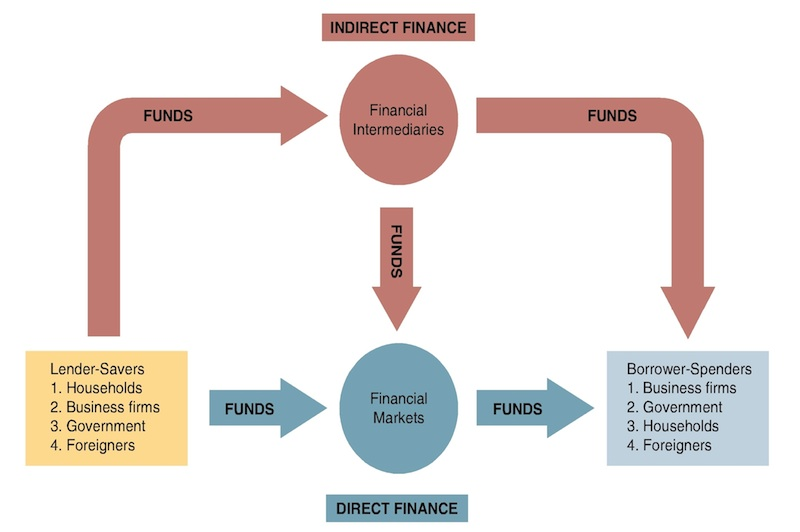
\includegraphics[scale=0.5]{./imgs/21.jpg}
\ra Direct finance: borrowers borrow funds directly from financial markets by selling securities
\ra Indirect finance: a financial intermediary borrows funds from lender-savers and then uses these funds to make loans to borrower-spenders.
\ra Financial markets are critical for producing an efficient allocation of capital which contributes to higher production and efficiency for the economy as a whole.
\ra Structure of financial markets
\rn{1} Debt and Equity Markets
\rna Short-term less than a year. 1-10 years are intermediate. $>10$ is long-term 
\rna Firms or individuals can obtain funds through issuing debt instruments (bonds/mortgage) or issue equities (stock)
\rna A disadvantage of equities is the holder is a residual claimant, the firm must pay debt holders first before its equity holders. 
\rna A advantage to holding equities is the direct benefit of increased firm profits versus the fixed amounts of debt, because of ownership rights of equities.
\ra Brokers are agents of investors who match buyers with sellers, dealers link buyers and sellers by buying and selling at stated prices. 
\rn{2} Primary and Secondary Markets
\rna Primary market for initial issues of securities (Investment banks). 
\rna Secondary markets (JSE) make securities more liquid, also set benchmark prices for the primary market. 
\rn{3} Exchange and OTC markets
\rna Secondary markets.
\rna Exchanges, central location where buyers and sellers of securities conduct trades
\rna OTC dealers  at different locations sell securities to anyone willing to pay their prices. Similarly competitive to exchanges due to technology.
\rn{4} Money and Capital Markets
\rna Money market: short-term securities
\rna Capital markets: 1 year or greater.1

\ssh{Financial market instruments}

\ra Money market short-term debt instruments.
\rn{1} US Treasury Bills. Short-term, no interest payments, set payment at maturity, sold at a discount. Most liquid and safest. Mainly held by banks.
\rn{2} Negotiable Bank Certificates of Deposit: a certificate of deposit (CD) is a debt instrument sold by a bank to depositors that pays annual interest of a given amount and at maturity pays back the original price. Negotiable CD’s are traded in secondary markets.  Big source of funds for banks.
\rn{3} Commercial Paper is a short-term debt instrument issued by large banks and well-know corporations.
\rn{4} Repurchase agreements are effectively short-term loans less than 2 weeks for which Treasury bills serve as collateral. Big source of funds for banks. Issued mainly by corporations.
\rn{5} Federal Funds, overnight loans between banks using their deposits at the Federal reserve.
\vspace{6pt}
\ra Capital Market for longer term debt.(Riskier than money market) 
\rn{1} Stocks. Largest security in capital market, Held by households and institutions.
\rn{2} Mortgages are loans to households or firms to purchase housing, land or real structures that serve as collateral. Largest debt market in US. 
\rna  Mortgage back security is a bond like instrument backed by a bundle of individual mortgages whose interest and principle payments are collectively paid to the holder-of the security.
\rn{3} Corporate Bonds. Issued by corporations with strong credit ratings. Convertible bonds can be changed into stock anytime up till maturity. Principle buyers are life insurance, pension funds households and other large holders. Not as liquid as government securities. Larger than new stock issues.
\rn{4} US Government Securities. Most liquid security.
\rn{5} US Government Agency Securities
\rn{6} State and Local Government Bonds (Municipal bonds). Issued by state and local governments for big projects, exempt for income tax. Banks largest holders.
\rn{7} Consumer and Bank Commercial Loans.

\ssh{Indirect finance and 4 financial intermediary functions}
\ra The basic function of financial markets is to channel funds from savers who have excess funds to spenders who have a shortage of funds. 
\ra Direct finance is when borrowers borrow funds directly from lenders by selling them securities
\ra The process of indirect finance using financial intermediaries is call financial intermediation.
\ra More important source of funds for corporations than securities markets.
\ra Financial intermediaries are financial institutions that acquire funds by issuing liabilities and, in turn use those funds to acquire assets by purchasing securities or making loans.
\ra Indirect finance involves an intermediary that stands between lenders and borrows and helps transfer funds from one to the other. 

\ssh{Transaction Costs / Liquidity services}
\ra Time and money spent in carrying out financial transactions.  
\ra Intermediaries can reduce transaction because they benefit from economies of scale due to expertise and size. 
\ra Intermediaries provide liquidity services that make it easier for customers to conduct transactions. e.g Checking accounts to pay bills.

\ssh{Risk sharing}
\ra They sell less risky investment and then use the funds to purchase more risky investments. 
\ra They earn profit on the difference between the returns on risky assets they bought and the payments made on assets they sold. Also called asset transformation. 
\ra They help individuals to diversify and thereby lower the amount of risk through low costs and assets pooling.

\ssh{Asymmetric information}
\ra One party does not know enough about the other party to make accurate decisions.
\ra Intermediaries are better equipped and can alleviate asymmetric information problems. 
\ra Two forms
\rn{1} Adverse selection
\rna Occurs before the transaction
\rna Potential borrowers who are the mostly like to produce an undesirable outcome are the ones who most actively seek out a loan and are thus most likely to be selected. 
\rna Results in fewer loans to all as lenders hesitate to lend at all.
\rn{2} Moral hazard
\rna Occurs after the transaction. 
\rna The risk that the borrower will engage in activities undesirable to the lender hence increase in chance of default. 
\rna Reduces loans for all due hesitation to lend.
\rna If there were no asymmetric information there could still be a moral hazard problem because the lender knows there might be a default and reducing such risk is too costly, therefore still a moral hazard.
\ra Intermediaries are better equipped to screen out bad risk (reduce adverse selection) and monitor borrowers (reduce moral hazard)

\ssh{Economies of scope} 
\ra Lowering the cost of information production for each service by applying one information resource to many different services.
\ra Credit risk evaluation on corporation for loan and then sale of the corporation's bonds to the public.
\ra Creates conflict of interest (moral hazard problem) due to offering multiple services, and by information being concealed or misleading.

\ssh{Type of financial intermediates}
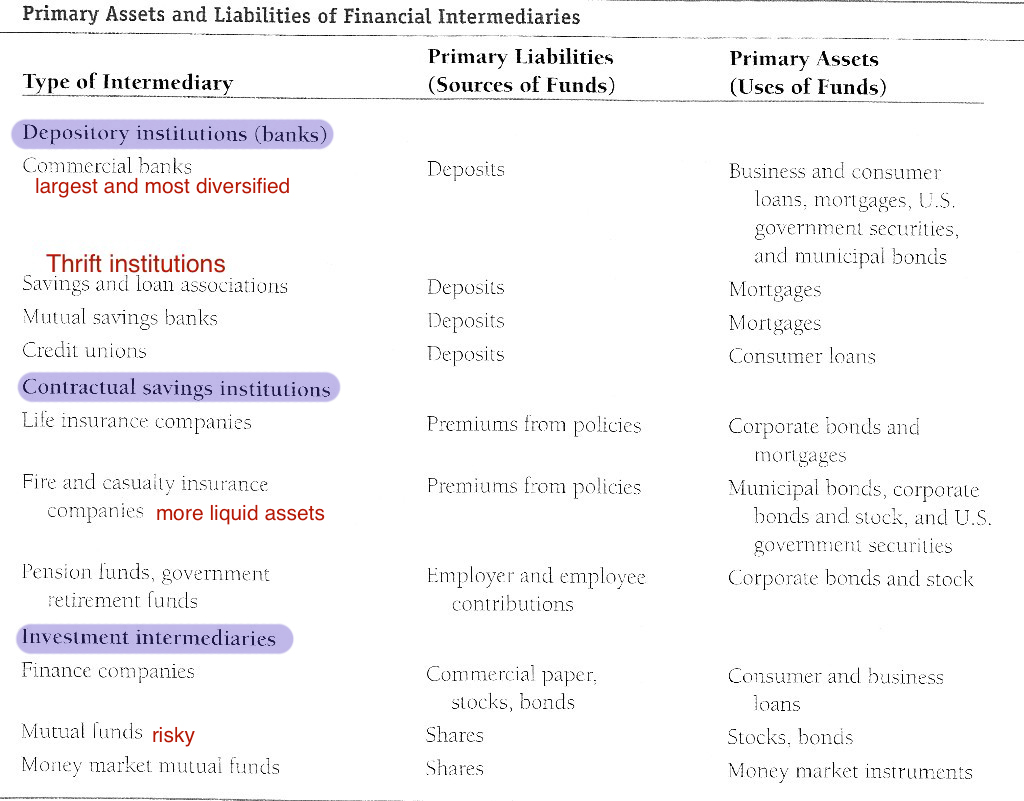
\includegraphics[scale=0.5]{./imgs/22.jpg}
\ssh{Investment banks}
\ra Don't take deposits. 
\ra Advises corporations on type of security to issue and then purchase the security at a predetermined price and resells on the market (underwriting). 
\ra Act as deal makers and earn fees on mergers and acquisitions.

\ssh{Regulation of the financial system}
\ra To reduce asymmetric information problems
\rn{1} Increase information available to investors 
\rna Provisions of information is improved by requiring companies issuing securities to report details about assets and liability, earnings, sales of stock 
\rna Preventing insider trading. 
\rn{2} Ensure the soundness of the financial system. 
\rna Soundness is ensured by restrictions on entry, disclosure, restrictions on assets and activities, deposit insurance, limits on competition and restrictions on interest rates.


%%%%%%%%%%%%%%%%%%%%%%%%%%%%%%%%%%%%%%%
\sh{Chapter 3: What is money}

\ssh{Meaning of money}
\ra Money is defined as anything that is generally accepted in payments for goods or services or in repayment of debts.
\ra It is measured as currency plus deposits. Money = Currency + Deposits
\ra Currency is paper money and coins
\ra Wealth is the total collection of pieces of property that serve to store value such as bonds, art, land, houses and cars.
\ra Income is the flow of earning per unit of time.
\ra Money is a stock variable. 

\ssh{Functions of money}
\rn{1} Medium of exchange
\rna Solves the double coincidence of wants (finding some one who has what you want at the same time  they want what you have), leads to high transaction costs.
\rna Money promote efficiency by eliminating time spent exchanging goods and services
\rna Encourages specialisation and division of labour.
\rna Money reduces transaction costs.

\rn{2} Unit of account 
\rna It is used to measure value in the economy
\rna Lowers transaction costs by reducing the number of prices that need to be considered.

\rn{3} Store of value
\rna A repository of purchasing power over time and enables delayed purchasing.
\rna Money is the most liquid asset of all because it is a medium of exchange as it does not need to be converted to anything else.
\rna Not the most attractive store value and depends on the price level.
\rna During inflation less money is held.

\vspace{6pt}
\ra For a commodity to function as money it must be:
\rn{1} Easily standardised to ascertain value.
\rn{2} Widely accepted
\rn{3} It must be divisible
\rn{4} Easy to carry
\rn{5} Not deteriorate quickly

\ssh{Evolutions of payment systems}
\rn{1} Commodity money
\rna Made up of precious metals such as gold and silver
\rna From ancient times to several hundred years ago
\rna Problem is the form of money is heavy and hard to transport
 
\rn{2} Fiat money
\rna Paper currency decreed by governments as legal tender but not convertible into coins or precious metals.
\rna Advantage is that it is lighter then coins or precious metal
\rna  Can on be accepted as medium of exchange if there is trust in authorities and extremely difficult to counterfeit.
\rna Easy to change currency due to the legal guarantee, e.g. Euro.
\rna Disadvantages is easily stolen, and expensive to transport in large amounts because of bulk.

\rn{3} Checks
\rna An instruction from your bank to transfer money from your account to another account when check is deposited.
\rna Don't need to carry around large amounts of currency
\rna Frequent back and forth payments cancel out.
\rna Reduces transportation costs and improves economic efficiency.
\rna Make large payments much easier
\rna Reduced the possibility of theft because they proved receipts for purchases.
\rna Takes time for checks to get from one place to another.
\rna Takes a few days to clear payment in check account.
\rna Processing checks is costly.

\rn{4} Electronic payment
\rna Electronic transfer payments due to adoption of cheap computers and internet.
\rna Allows recurring automated payments
\rna Large cost savings over using checks.

\rn{5} E-money
\rna Money that exist only in electronic form.
\rna Debit cards allows consumers to purchase goods and services electronically.
\rna Store-value card are repurchased for specific amounts.
\rna Smart cards contain chips and are loaded with cash from a bank account when needed.
\rna e-cash is used on the internet to purchase goods, and is money transferred to a PC from a bank and secured by cryptography..
\rna Cryptocurrencies like bitcoin secured by cryptography and proof of work scripts. 

\ssh{Notes on credit exclusion from $M=C+D$}
\ra Not all forms of credit are counted as money. 
\ra Two forms of credit.
\rn{1} Credit cards held by consumers. 
\rna Credit cards normally provide credit up to some limit
\rna  The credit provided only have to be settled at a later stage
\rn{2} Trade credit.
\rna  Trade credit is when firms sell their products to the trade sector, on condition that payment for the goods is made at a future date
\ra Credit in both these two forms serves as a medium of exchange, but these forms of credit do not lead to an increase in cash or deposits, and the money stock is not affected.
\ra Not included because of difficulties in measuring these forms of credit. 
\ra The provision of trade credit, for example, may lead to indirect increases in money supply.

\ssh{Measuring money in SA }
\ra Defined as currency plus deposits held by domestic, private nonbank sector at commercial banks.
\ra In South Africa currency is all the paper money and coins in circulation less cash held in bank vaults. \ra $M=C+D$
\ra Deposits are all domestic private non-bank deposits in banks and excludes:
\rn{1} Government deposits at commercial banks  
\rn{2} Foreign bank deposits at commercial banks
\rn{3} Cash held by banks themselves (vault cash), Excluded because they are not available for spending by the private sector and cannot function as a medium exchange.
\ra Economic transactions in principle do not affect the money stock.
\ra The amount of currency in circulation is known since only the central bank issues currency. 
\ra Because deposits are always held at banks, banks know the exact amount of deposits held by the non-bank (private) sector.
\ra Monetary authorities: SARB and the CPD (Corporation for public deposits) 
\ra Commercial banks. Only registered banks and mutual banks, the Landbank and the Postbank are classified as other depository institutions.

\ssh{Monetary aggregates}
\ra Stock variables measured at month end.
\rn{1} M1A 
\rna Consists of cash (coins and banknotes) + cheque and transmission deposits 
\rna Cheque and transmission deposits are no interest deposits mainly used to make payments. 
\rna If interest rate rises on medium to long-term deposits there will be a transfer into medium to long-term deposits.
\rna In SA constituents small portion of M3

\rn{2} M1 Narrow definition.
\rna M1A + other demand deposits by private sector.
\rna Other demand deposits are monetary deposits other than transaction or chequeable deposits.
\rna Other demand deposits are deposits that are convertible into cash on demand, and normally carry a payment facility.
\rna High interest rates on other assets, means opportunity cost of keeping funds in monetary demand deposits is high, and funds are shifted to interest-bearing deposits.
\rna In SA constituents large portion of M3

\rn{3} M2 
\rna a broader definition of money
\rna M1 + plus deposits
\rna Includes short-term (1 to 31 days) and medium-term deposits (32-180 days) such as savings deposits, savings bank certificates, "share" investments, negotiable certificates and promissory notes.
\rna Cannot be converted into cash on demand, but only after some time, does not carry a payment facility.
\rna Near money, because terms are short and they are closely related and substitutes for demand monetary deposits in M1, 
\rna They are liquid.
\rna In SA constituents large portion of M3

\rn{4} M3
\rna The most comprehensive measure of money
\rna M2 + long-term deposits.
\rna Includes all monetary and non-monetary deposit liabilities of the monetary banking sector.
\rna Long terms deposits are relatively liquid.
\rna Because it involves considerable effort and cost to move funds between the components of M3 and financial assets that do not form part of M3, the M3 monetary aggregate is much more stable than its components, and is a much better indicator of domestic spending.

\ssh{What causes money stock to increase}
\rn{1} Bank loans to private nonbank sector (Most important)
\rn{2} Transactions in financial assets between the banking sector (central and commercial banks) and the private nonbank sector
\rn{3} Government transactions with the private nonbank sector
\rn{4} Foreign exchange transactions

\textbf{Implications of the government printing money}
\ra Two types:
\rn{1} Printing banknotes and coins to finance expenditure. 
\rna Only SARB has the right to print money.
\rna SARB prints money and sells it to banks (replaces old notes and for private sector cash requirements {\bf Vault Cash}). The SARB profits (Income less costs) are then transferred to government bank accounts. No increase in money supply (Government deposit excluded).
\rna Government then spends money and private sector deposits increase, therefore money supply increases.
\rna Normally not a problem (cash component small proportion of total money stock)  unless government is corrupt and abuses the processes creating excess money.
\rn{2} Government forces the central bank to buy excessive issues of government securities
\rna Monetisation of government debt.
\rna Central banks are not independent enough
\ra MV+PY and therefore an increase in money stock causes an increase price level.
\ra Hyperinflation occurs when, over the medium to long term, a vicious cycle of (money creation \ra   inflation \ra money creation) occurs.. 
\ra In Zimbabwe it destroyed both the financial sector and the economy,  caused untold hardship and misery to the population, with the poor, being unable to protect themselves against the ravages of high inflation, suffering most.

%%%%%%%%%%%%%%%%%%%%%%%%%%%%%%%%%%%%%%%
\h{Part 2}
\sh{Chapter 4: Understanding interest rates}

\sh{Measuring Interest Rates}

\ra Present value (PV) a dollar paid to you one year from now is less valuable than a dollar paid today because you can earn interest on a dollar today. Enables comparing the values of credit instruments with different payment timings.

\ssh{4 types of credit market instruments}
\rn{1} Simple loan such as many money market instruments.  Borrowed funds repaid at maturity with additional interest payment. 
\rna Simple interest rate equals yield to maturity = NPV.
\rn{2} Fixed-payment loan (fully amortised loan), same payment every month, which includes interest and principal, such as mortgages. 
\rna Yield to maturity = IRR.
\rn{3} Coupon bond, pays a fixed coupon payment every year until maturity when face/par value is repaid, such as us treasury bonds, corporate bonds. Identified by 4 pieces of information: Face value, issuing agency, maturity date, coupon rate. Yield to maturity = IRR. 
\rna Priced at face value, then yield to maturity = coupon rate.
\rna Price of a coupon bond and yield to maturity are negatively related, when the interest rate rises, the price of the bond falls. 
\rna The yield to  maturity is greater than the coupon rate when the bond price is below its face value. 
\rna  {\bf Perpetuity (consol) bond}, has no maturity date and no repayment of principle, and that makes fixed coupon payments forever.
\rna Current Yield is yearly coupon payment divided by the price of the security.
\rn{4} Discount bond, (zero coupon bond) bought at a discount of it face-value and then repaid at face value at maturity, us treasury bills, savings bonds. No interest payments.  
\rna Yield to maturity is the increase in price over the year divided by the initial price.
\rna Can have negative interest rates and purchasing power is not fully compensated.
\rna The yield to maturity is negatively related to the current bond price.

\ssh{Yield to maturity}
\ra The interest rate that equates the present value of cash flow payments received from a debt instrument with its value today.
\ra Makes good economics sense and therefore most accurate measure of interest rates.

\ssh{The distinction between interest rates and returns}
\ra Rate of capital gain is the change in the bond's price relative to the initial purchase price.
\ra Return on a bond is the current yield + rate of capital gain.
\ra Rate of return is defined as the payments to the owner plus the change in value, expressed as a fraction of its purchase price.
\ra The return on a bond will not necessarily equal the yield to maturity on that bond, due to price fluctuations giving higher or lower capital gains. 
\ra Prices and returns for long-term bonds are more volatile than those of shorter term bonds. 
\ra The only bond whose return equals the initial yield to maturity is one whose time to maturity is the same as the holding period.
\ra A rise in interest rates is associated with a fall in bond prices, resulting in capital losses on bonds whose terms to maturity are longer than the holding period.
\ra The more distant a bond's maturity, the lower the rate of return that occurs as a result of the increase in the in the interest rate. 
\ra The more distant a bond's maturity, the greater the size of the percentage price change associated with an interest rate change.
\ra Paper loss if bond is not sold.

\ssh{Interest rate risk} 
\ra Prices and returns for long-term bonds are more volatile than those for shorter-term bonds due the sensitivity of longer term bonds to interest rate changes. 
\ra Due in lager fact to the term to maturity being more than the holding period.
\ra Bonds with a maturity that is as short as the holding periods have no interest rate risk.
\ra Reinvestment risk: when the holding period is longer than the term  to maturity of a bond, due to uncertain future interest rates when reinvestment men occurs.

\ssh{The distinction between real and nominal interest rates}
\ra Real interest rate: nominal rate less expected inflation. $r=i-\pi^e$ 
\ra Real interest rate reflects the real cost of borrowing.
\ra ex ante real interest rate is before the fact and ex post real interest rate is after the fact.
\ra When the real interest rate is low there are greater incentives to borrow and fewer incentives to lend. 
\ra Real returns which indicate the amount of extra goods and services that can be purchased.
\ra Real interest rates are a more accurate indicator of the tightness of credit market conditions. 

\ssh{Indexed bonds} 
\ra Interest and principal payments are adjusted for changes in the prices level. 
\ra Provide a direct measure of a real interest rate.
\ra They are useful because to monetary policy makers because subtracting their interest rates from a nominal rate on a non-indexed bond, they give insight into expected inflation.

%%%%%%%%%%%%%%%%%%%%%%%%%%%%%%%%%%%%%%%
\sh{Chapter 5: The behaviour of interest rates}
\ssh{Determinants of asset demand}
\ra Wealth: total resources owned by an individual. including all assets.
\ra Expected Return: the return expected over the next period on one asset relative to another.
\ra Risk: the degree of uncertainty associated with the return on on asset relative to alternatives.
\ra Liquidity: the ease and speed with which an asset can be turned into cash relative to other assets.

\ssh{Theory of Portfolio choice} 
\ra How much of an asset people want to hold in their portfolios. An states the facts in the table below. 
\vspace{6pt}
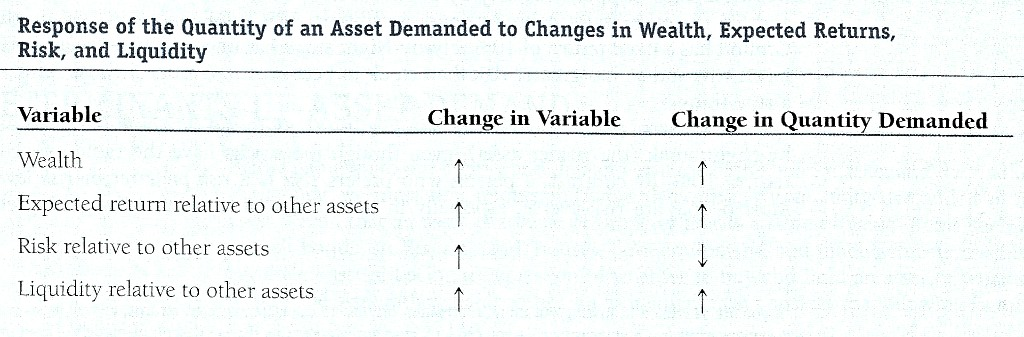
\includegraphics[scale=0.5]{./imgs/50.jpg}

\ssh{Supply and demand in the bond market}
\ra  Demand curve, relationship between quantity demanded and price or interest rate. It has a downward slope indicating lower prices for the bond the quantity demand is higher, ceteris paribus. Lenders of funds.
\ra Supply curve, relationship between quantity supplied and price, ceteris paribus. Higher prices means higher supply. Borrowers of funds. The higher the price of bonds, the more the borrower receives and the lower the interest rate which the borrower must pay.
\ra Market Equilibrium. Clearing price. Quantity of bonds demanded equals quantity of bonds supplied. The market head towards this point and settles. $\rm{B^d}=\rm{B^s}$
\ra Excess supply, people want to sell more bonds than others want to buy. 
\ra Excess demand, people want to buy more bonds than others want to sell. 
\ra The asset market approach does demand and supply analysis in terms of stocks of assets and not flows, due to the inherit difficulty of flows especially in the face of inflation.
\ra If households save more, wealth increases.

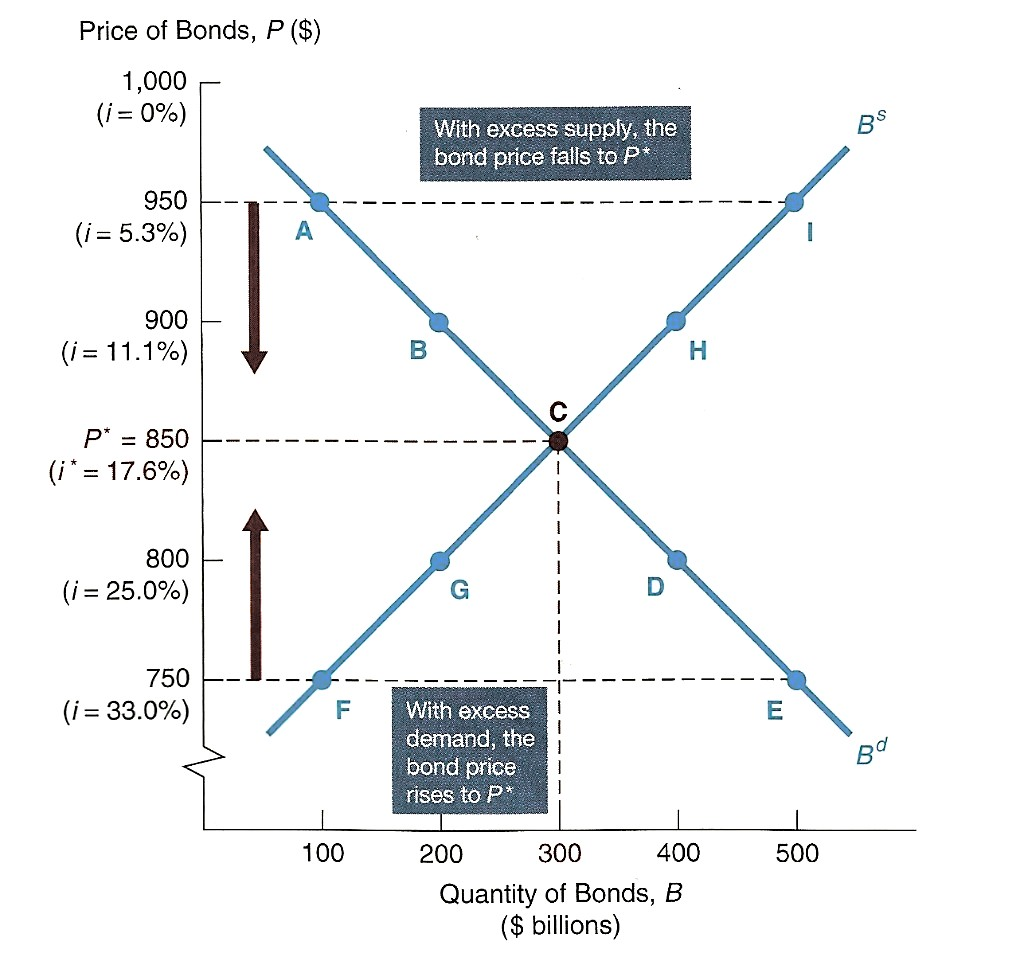
\includegraphics[scale=0.3]{./imgs/51.jpg}

\ssh{Changes in Equilibrium interest rates}
\ra Simpler analysis of effects from changes in inflation.
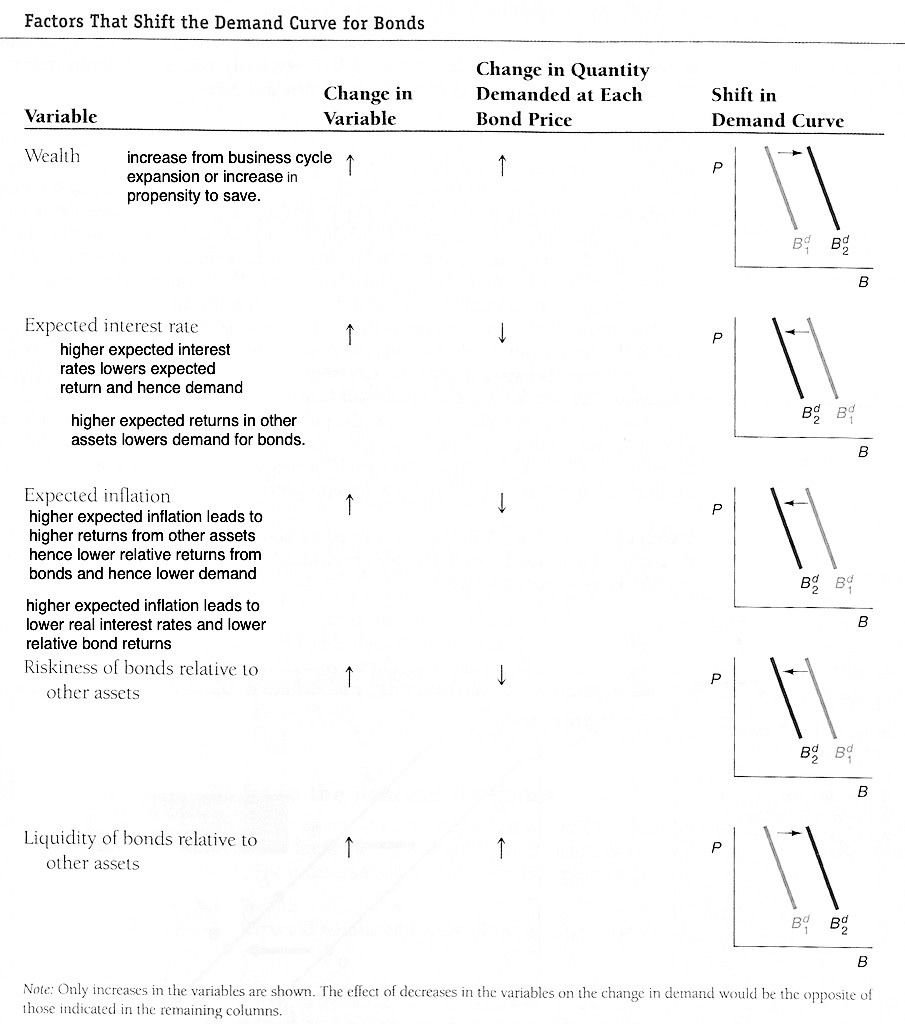
\includegraphics[scale=0.5]{./imgs/52.jpg}
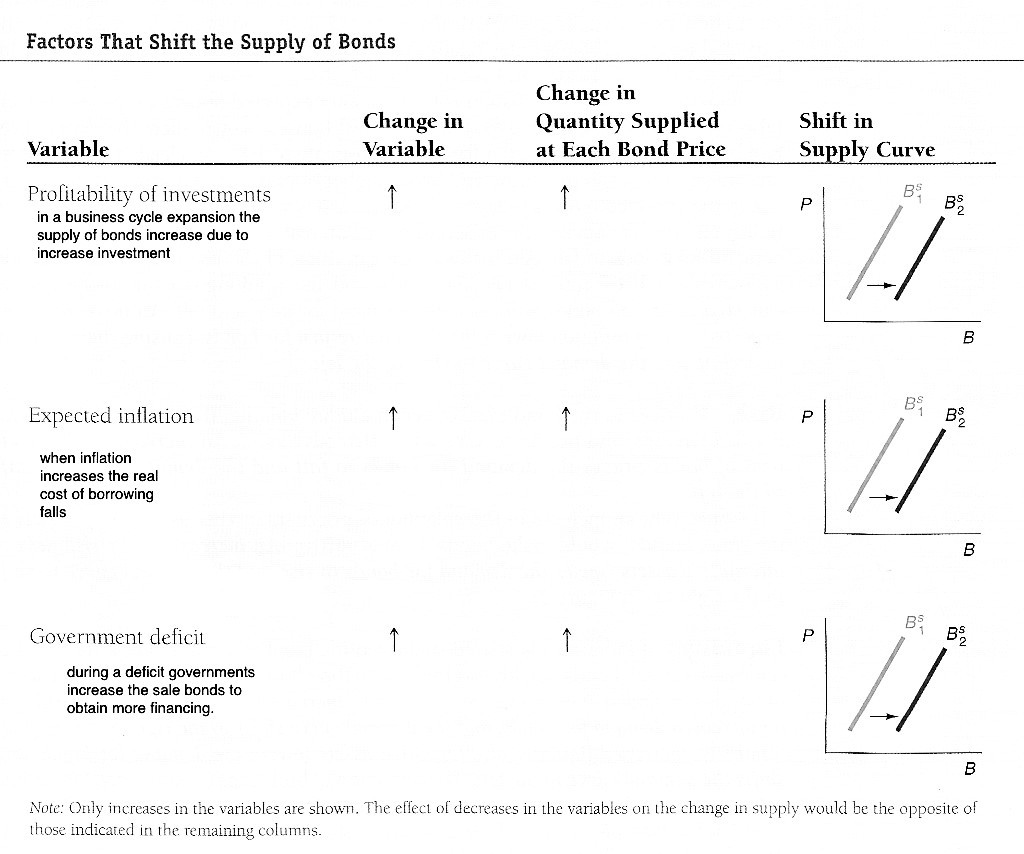
\includegraphics[scale=0.45]{./imgs/53.jpg}

\ssh{Changes in the interest rate due to expected inflation, the Fisher Effect}
\ra When expected inflation rises, interest rates will rise, also called the Fisher Effect. 
\ra Ambiguous change in quantity, but certain increase in interest rate.
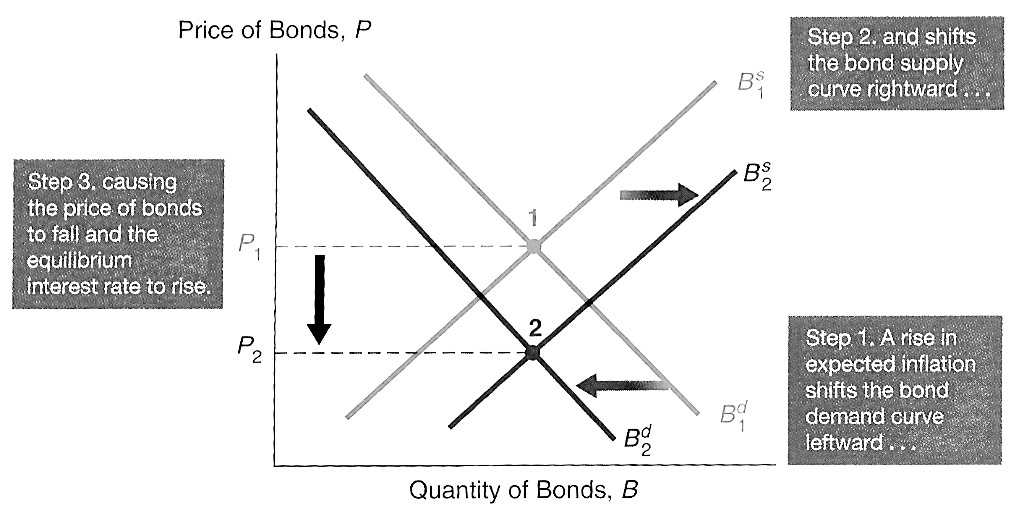
\includegraphics[scale=0.4]{./imgs/54.jpg}

\sh{Changes in the interest rate due to a business cycle expansion}
\ra Amounts of goods and services rise with a corresponding increase in national income and business has more opportunities to expand, therefore they increase the supply of bonds.
\ra An increase in wealth will, via the theory of portfolio choice, increase the demand for bonds. 
\ra Ambiguous change in interest rate but certain increase in quantity.
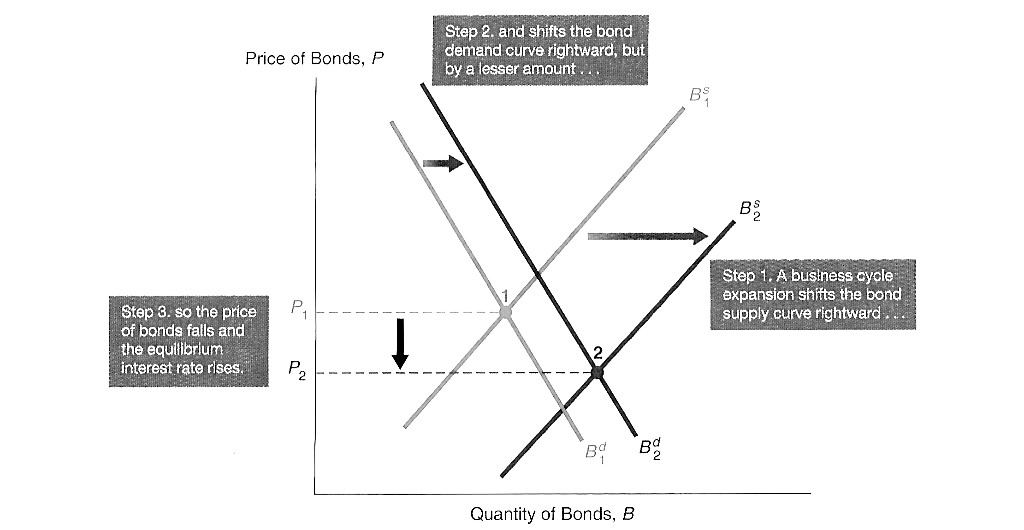
\includegraphics[scale=0.4]{./imgs/55.jpg}

\ssh{Supply and demand in the market for money: The liquidity preference framework}
$\rm{B^S+M^S=B^d+M^s}$ or $\rm{B^S-B^d=M^d-M^s}$
\ra Simpler analysis is of effects from changes in income, price level and supply of money.
\ra Simplifying assumptions: 
\rn{1} Assumes there are only two kinds of assets, money and bonds which equals total wealth, and therefore implicitly ignores any effects on interest rates from changes in expected returns on real assets such as cars. 
\rn{3} Assumes money has a zero rate of return as it earns no interest. Supply curve is vertical which is not the case in South Africa.
\ra Demand curve: As the interest rate rises the expected return of money relative to bonds falls and the demand for bonds increases. The quantity of money demand and interest rate are negatively related because of the rising opportunity costs of holding money when interest rates are increasing.
\ra Supply curve: Central bank supplies a fixed quantity.
\ra Equilibrium: $\rm{M^s=M^d}$ at the intersection of the supply and demand curves.
\ra When the price level increases more money will be demanded to restore purchasing power.

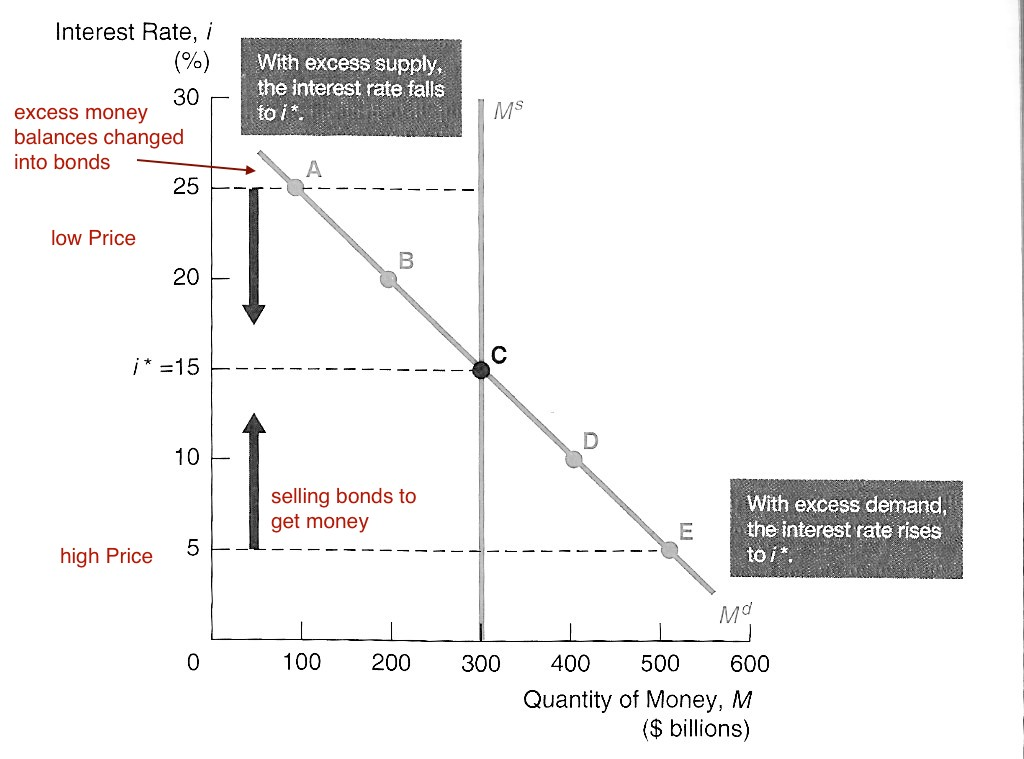
\includegraphics[scale=0.3]{./imgs/56.jpg}

\ssh{Changes in Equilibrium interest rates in the LPF}
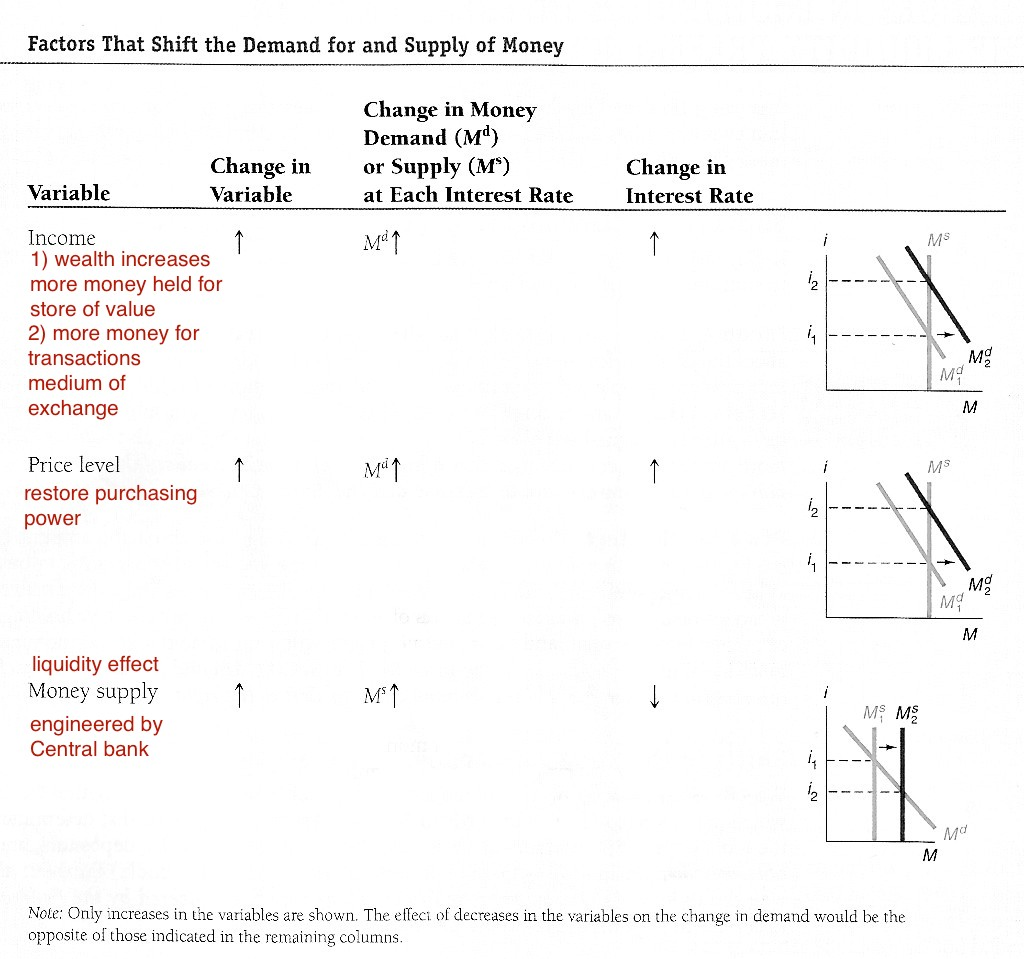
\includegraphics[scale=0.35]{./imgs/57.jpg}

\ssh{3 effects of changes in money supply} 
\rn{1} The income effect of an increase in the money supply is a rise in interest rates in response to the higher level of income.
\rn{2} the price-level effect from and increase in the money supply is a rise in interest rates in response to the rise in price level.
\rn{3} the expected-inflation effect of an increase in money supply is a rise in interest rates in response to the rise in the expected inflation rate. The expected-inflation effect will persist only as long as the price level continues to rise.
\ra Basic difference between price-level effect and expected-inflation effect is that the price-level effect remains even after prices have stopped rising whereas the expected inflation effect disappears.

\ssh{Response over time to an increase in money supply growth}

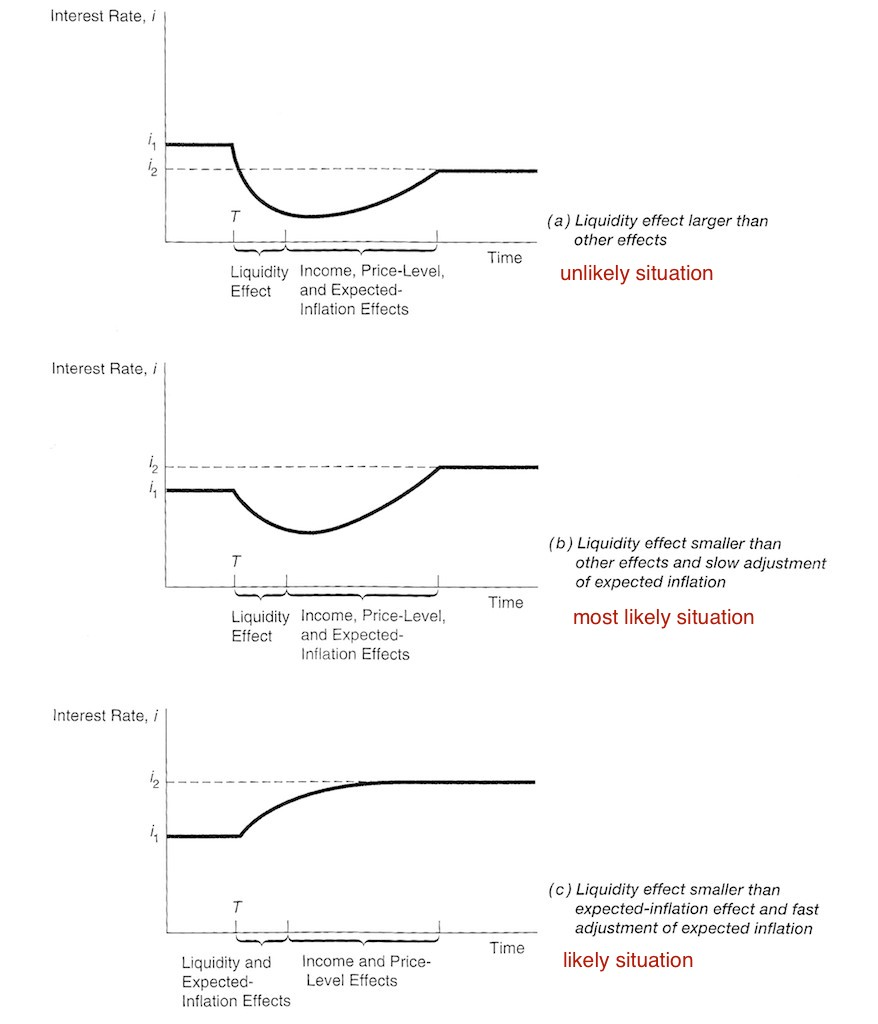
\includegraphics[scale=0.5]{./imgs/58.jpg}


%%%%%%%%%%%%%%%%%%%%%%%%%%%%%%%%%%%%%%%
\sh{Chapter 6: The risk and term structure of interest rates}

\ssh{Risk structure of interest rates.}
\ra The risk structure of interest rates is the relationship among interest rates on bonds with the same maturity.
\ra 3 Factors affecting risk structure 
\rn{1} Default risk. 
\rna Default risk is the risk of the issuer of the bond being unable or unwilling to make interest payments or pay off the face value when the bond matures.  
\rna Bonds are such as US Treasury bonds are considered {\bf default free}, as they are backed by the US government which can increase taxes or print money to meet it obligations. 
\rna The {\bf risk premium} is the difference between bonds with default risk and bonds that are default free. 
\rna A bond with default risk will always have a positive risk premium 
\rna Increase in default risk will raise the risk premium. 
\rna Credit ratings agencies provide information about the likelihood of a bond issuer defaulting. They can have conflicts of interest in both structuring debt instruments and selling them. Junk bonds have high risk premium but are high-yield bonds.

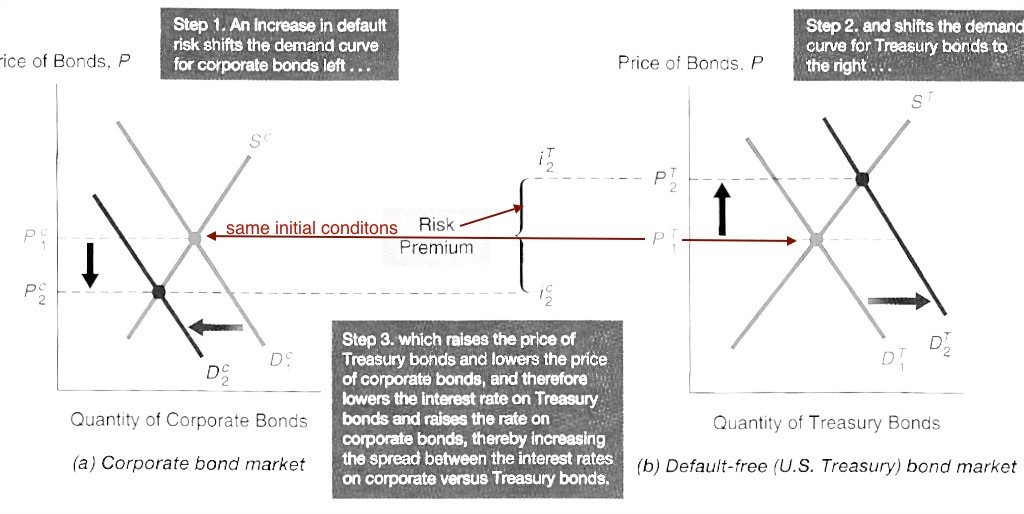
\includegraphics[scale=0.45]{./imgs/61.jpg}

\rn{2} Liquidity 
\rna the higher the bond's liquidity the more appealing it is and therefore there would be a rightward shift in the demand for bonds curve.
\rna  US Treasury bonds are the most liquid of all bonds. 
\rna Same graph as default risk case.

\rn{3} Income tax considerations. 
\rna Bonds that are exempt from tax have higher expected returns and hence there is an increased demand for them.
\rna Bonds with tax free interest payments have lower interest rates.
\rna Municipal bonds are not default free and not as liquid as treasury bonds.

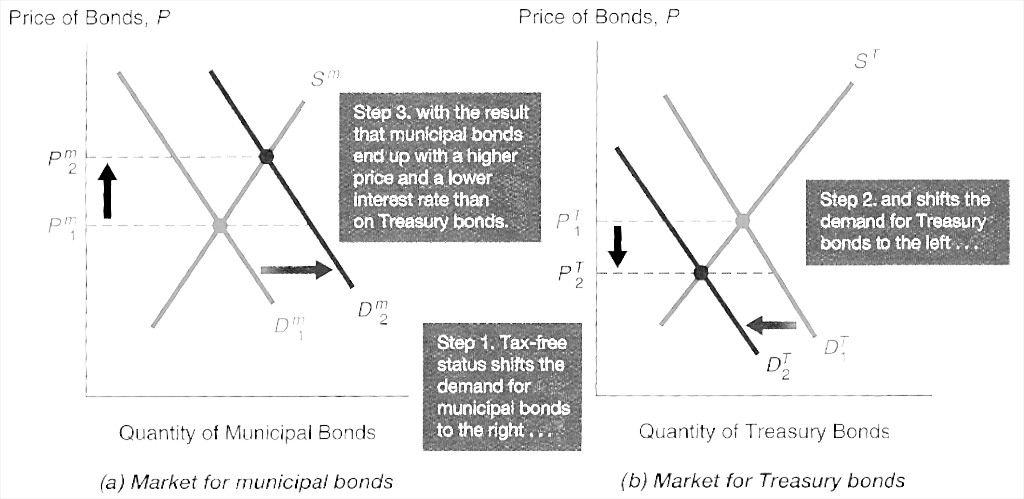
\includegraphics[scale=0.45]{./imgs/62.jpg}

\ssh{Term structure of interest rates and the yield curve.} 
\ra Bonds with identical risk, liquidity and tax characteristics may have different interest rates because their time remaining to maturity is different. A plot of the yield is called a yield curve. 
\ra Upward sloping yield curves (usual case)indicate long-term interest rates are higher than short term interest rates. 
\ra Flat yield curves mean same short and long-term interest rates
\ra Downward (inverted) sloping yield curves mean long-term rates are below short-term rates.
\ra Yield can also have more complex shapes as in up and down.

\ssh{3 empirical facts to be explained}
\rn{1} interest rates on bonds of different maturities move together over time. Explained by Expectations and liquidity premium theories.
\rn{2} when short-term interest rates are low, yield curves are more likely to have an upward slope and when short-term rates are high yield curves will be inverted. Explained by Expectations and liquidity premium theories.
\rn{3} yield curves almost always slope upward. Explained by Segmented, and liquidity premium theories.

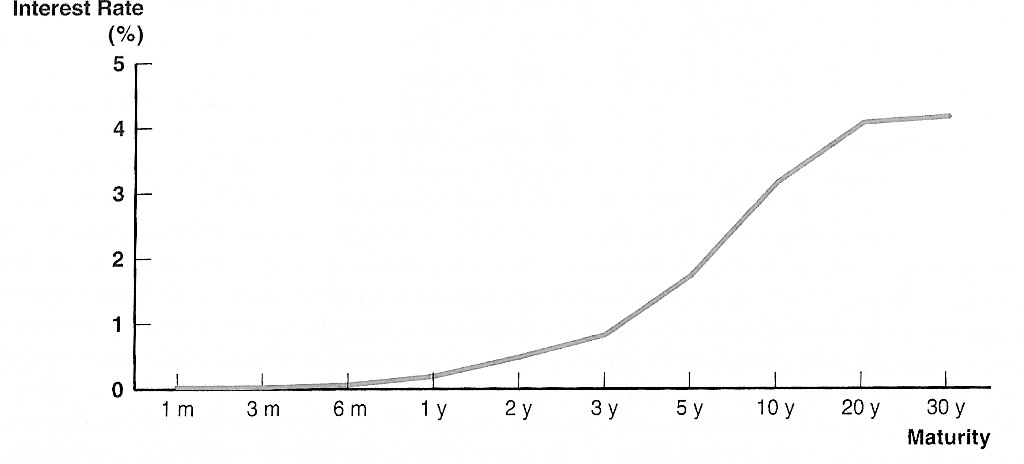
\includegraphics[scale=0.3]{./imgs/65.jpg}

\ssh{Expectations theory}
\ra The interest rate on a long term-term bond will equal an average of the short-term interest rates that people expect to occur over the life of the long-term bond. 
\ra The key assumption is that buyers of bonds do not prefer bonds of one maturity over another, so they will not hold any quantity of a bond if its expected return is less that that of another bond with a different maturity
\ra Implies Bonds with different maturities are perfect substitutes therefore same expected return. 
\ra When the yield curve is upward sloping short term interest rates are expected to rise. Or the average of expected future short-term rates is higher than the current short-term rate.
\ra When the yield curve is inverted the average of future short-term interest rates is expected to be lower than the current short-term rate, implying that short-term interest rates are expected to fall. 
\ra If the yield curve is flat short-term interest rates are not expected to change on average in the future.
\ra Explaining empirical facts:
\rn{1} A rise in short term rates will raise people's expectation of future short-term rates and given that long-term rates are an average of short-terms rate they to will rise and hence move together.  \rn{2} When short term rates are low people will expect them to rise in the future and hence the average of future short-term rates rate is will be higher relative to the current short-term rates hence long-terms rates will bi higher and the yield curve has an upwards slope. Conversely for the high short-term rates and the inverted yield curve. 
\rn{3} It cannot explain this fact as it predicts a typical curve would be flat because a rise or fall in interest rates is equally likely.

\ssh{Segmented market theory}
\ra Sees markets for different-maturity bonds as completely separate and segmented no substitution and no effect on each other expected returns.
\ra Bond are not substitutes at all due to the fact that investors have a strong preference for bonds of one maturity but not for another and are only concerned with the expected returns of their preference. This is due to the preference for a certain holding period.  (holding period = term to maturity = no interest rate risk).
\ra The interest rate for each bond with a different maturity is then determined by supply and demand for that bond. 
\ra Explaining empirical facts:
\rn{1} Unable to explain fact due to the fact that different maturity bonds are segmented and have no influence on each others interest rates.
\rn{2} Unable to explain because it is not clear how demand and supply for short-term bonds versus long-terms bonds change with the level of short term interest rates. 
\rn{3} Demand for short-term bonds is higher due to the lower risk hence higher prices and lower interest rates and long term bonds have lower prices and higher interest rates. This explain the normal upward slope. 

\ssh{Liquidity premium theory and preferred habitat theory}
\ra Most widely accepted because explain facts the best and the other two theories lay ground work for this one, and shines a light on how economist modify theories to empirical evidence.
\ra The liquidity premium theory states the the interest rate on a long-term bond will equal an average of short-term interest rates expected to occur over the life of the long-term bond plus a liquidity premium (term premium) that responds to supply and demand. 
\rna Key assumption is that bonds of different maturities are substitutes with their expected returns influencing one another, they are not perfect substitutes.
\rna Investor tend to prefer short term bonds as they have lower interest-rat risk.
\rna Investor must be offered a positive liquidity premium to induce them to hold longer-term bonds.
\ra Preferred habitat theory assumes investors have preference for bonds of one maturity over another and will only buy non-preferred bonds with higher expected returns.
\rna Most investor prefer the shorter-term habitat and therefore longer  term bonds will have higher prices.
\ra Explaining empirical facts:
\rn{1} A rise in short-term interest rates mean short-term rates will be higher on average and therefore so will long-term rates and so they move together.
\rn{2} If short-term rates are high people expected them to come down, therefore average of future short term rates will be expected to be much more lower, therefore lower long-term rates (despite the liquidity premium) are lower and there is an inverted yield curve.
\rn{3} Because the liquidity premium rises with a bond maturity because of the strong preference for short-term bonds.
\begin{tabular}{p{0.5\textwidth} p{0.5\textwidth}}
  \vspace{0pt} \hspace{-30pt} 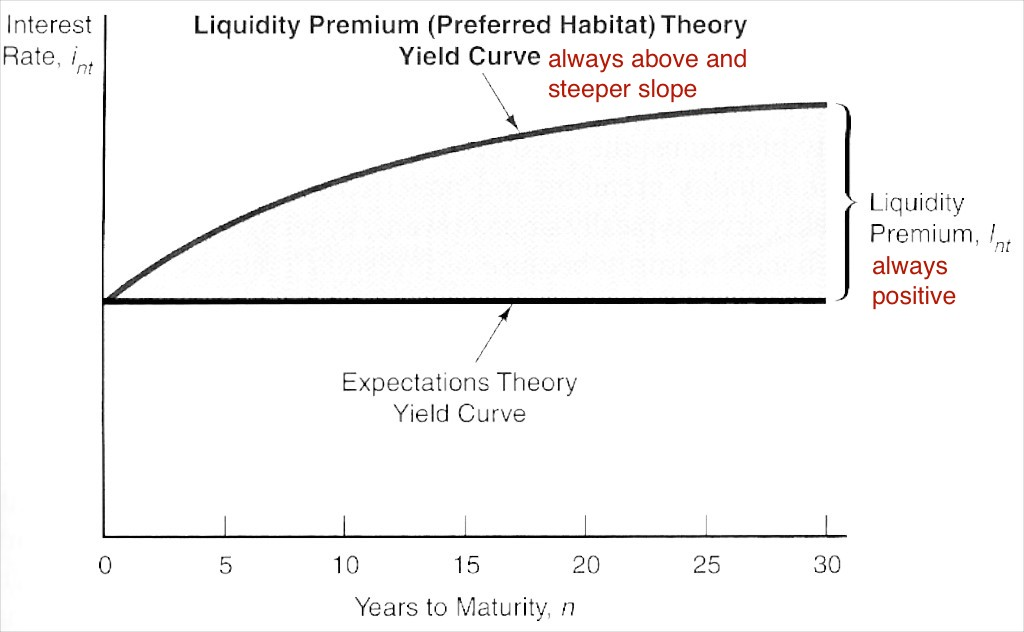
\includegraphics[scale=0.25]{./imgs/63.jpg}&
  \vspace{0pt} \hspace{-50pt} 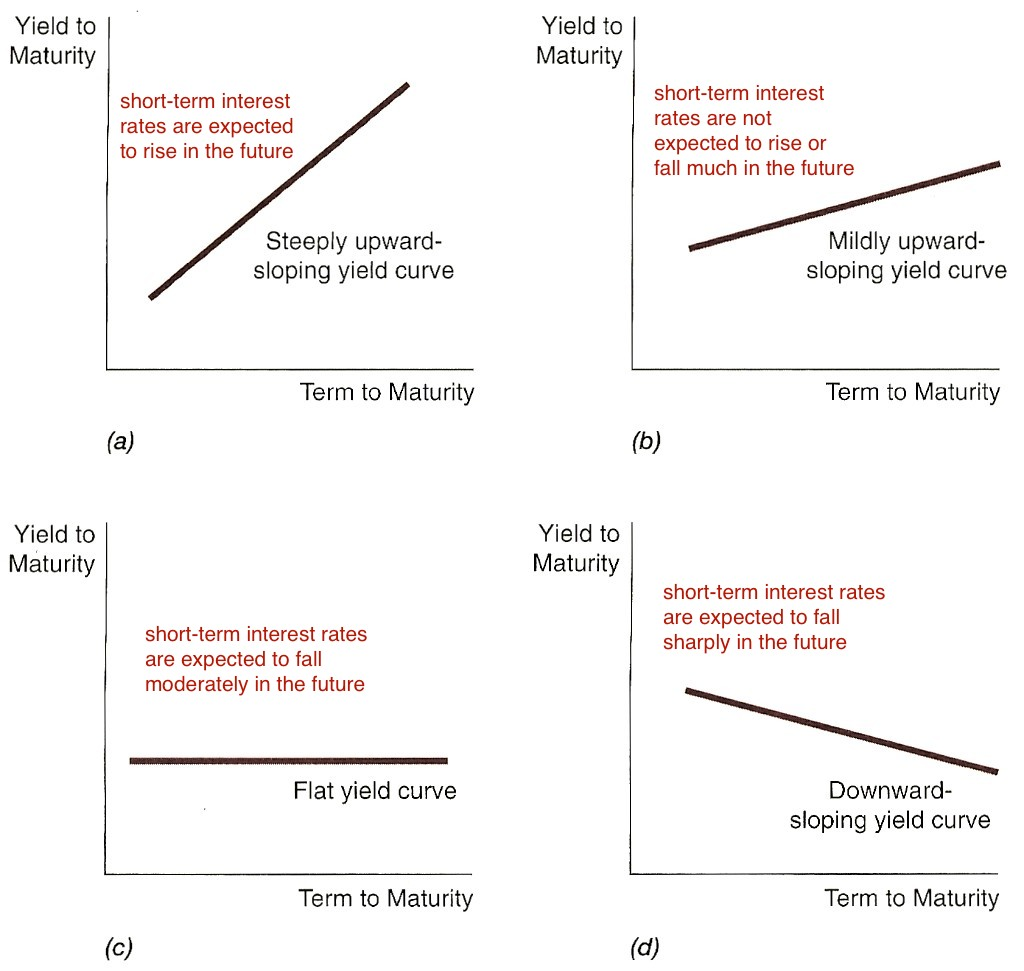
\includegraphics[scale=0.3]{./imgs/64.jpg}
\end{tabular}


\sh{Evidence of term structure}
\ra One test indicated spread between short and long-term does not always predict future interest rates because of fluctuations in the long term liquidity premium.
\ra New evidence suggests: Quite a bit of information in short-term and long-term structure, but unreliable at predicting rates over the intermediate term.
\ra Can also help forecast future inflation and business cycles.

\ssh{SA yield curve}
\ra Extremely volatile
\ra The short-term bond yield is heavily affected by monetary policy and the repo rate.
\ra The long-term bond yield is heavily affected by inflation, foreign exchange markets and the general economic outlook.

%%%%%%%%%%%%%%%%%%%%%%%%%%%%%%%%%%%%%%%
\h{Part 3}
\sh{Chapter 8: An Economic analysis of financial structure}

\ssh{How financial intermediaries reduce  transaction costs.}
\ra Financial intermediaries stand between lender-savers and borrow-spenders. 
\ra They enable funds to be transferred from people with non-productive opportunities to people with productive opportunities. 
\ra In financial markets the costs of transacting is high. 
\rn{1} Economies of scale
\rna They bundle investors funds together to reduce the cost per  individual investor.
\rna The costs of a small transaction are similar to the costs of a large transaction. 
\rna Example a Mutual fund financial intermediary which sells shares to individuals and then invests the proceeds in bonds and stocks. The charge fees for administrating accounts.
\rna They increase diversification of risk, buy purchasing a range of securities, as small investors would be compelled to keep all their eggs in the same basket, to keep costs down. 
\rna Economies of scale are important in lowering costs for communication and computerisation in financial transaction.
\rn{2} Expertise
\rna Expertises in things such as computer technology, providing help desks and information. 
\rna They provided liquidity services (easier transactions or being able to pay bills).

\ssh{Lemons problem and adverse selection}
\ra Buyers cannot asses the quality of used cars, therefore the price buyers will pay must reflect the average quality, between a low lemon and a high peach.
\ra The owners knows the quality of the used car
\rn{1} If its low (lemon) they will be happy to accept the average price which is higher than a lemon. 
\rn{2} If its high(peach) then the owner knows the car is undervalued at the average price and may not sell. 
\ra The result is fewer good cars and the average quality ill be low, hence few sales and a poorly functioning market.
\ra In the absence of asymmetric information where buyers know as much about the quality of the used car as the sellers then buyers will be willing to pay full value for good used cars.
\ra Because byers are getting a fair price they will sell, and the market will have many transactions.
\ra Similar arguments for stock and bond markets.
\vspace{6pt}
\ra{Tools to solve adverse selection problem}
\rn{1} Private production and sale of information
\rna Provide the people supply funds with more details  about the individuals or firms seeking finance.
\rna Private companies collect and produce information that distinguishes good from bad.
\rna Creates the free-rider problem, where people who don't pay for the information take advantage of the information other people have paid for.
\rna If A paid for info to invest in undervalued securities, and B and many others copy A, then the price will go up and the security will no longer be undervalued and hence A will not buy info in the future.
\rna The weakened ability of private firms to profit from selling information will lead to less information in the marker and an increase in adverse selection.
\rn{2} Government regulation to increase information
\rna Government would be reluctant to release negative information as it would be politicly unfavourable.
\rna Governments regulate securities markets to encourage firms to reveal honest and accurate information about themselves, and requiring audits. 
\rna Does not always work e.g. Enron. Statistics do not reveal the entire picture and bad companies tend to paint the information in a good light.
\rn{3} Financial intermediation
\rna They become experts in the production of information about firms and sorting the good credit risks from the bad ones.
\rna The higher profits from the information serves to incentivise information production.
\rna They avoid the free-rider problem by making private non-traded loans and not public purchases.
\rna Banks have an increased role in developing economies because they reduced adverse selection
\rna As information becomes easier to acquire the role of banks will decline.
\rna Easier for bigger firms to get funds in the direct route as more information about them is available.
\rn{4} Collateral and net worth
\rna Reduces the lenders loss in the result of default and therefore reduces adverse selection
\rna Lenders are more willing to make loans because of the reduce risk.
\rna Borrowers are more willing to supply collateral to get the loans
\rna High net worth (difference between assets and liabilities) can serve as collateral

\ssh{Moral hazard and equity contracts}
Principal-agent problem (Moral hazed in equity contracts)
\ra Separation of ownership and control involves moral hazard, as managers (agents) may act in their own interests rather than in the interests of the stock-holders (principles) because the managers have less incentive to maximise profits than shareholders do.
\ra Examples are pursuing personal interests like diverting funds, or acquisitions of firms that increase personal power but do not increase profitability.
\ra Would not arise if owners had complete information about the mangers and could prevent wasteful or fraudulent expenditure.
\ra Would also not arise if there was no separation of ownership and control.
\vspace{6pt}
\ra{Tools to solve moral hazard problem in equity contracts}
\rn{1} Production of information: Monitoring (Costly state verification)
\rna Principles can monitor agents actions, conduct regular audits
\rna Can be expensive in terms of time and money and makes equity contracts less desirable.
\rna Subject to free-rider problem where if you know other stockholders are monitoring the agents then you can take a free ride on their activities, if everyone does this the moral hazard increases.
\rn{2} Government regulation to increase information.
\rna Governments have laws to force firms to adhere to standard accounting principles that make profit verification easier. 
\rna The impose criminal penalties for fraud and theft.
\rna Only partly effective as fraud detection is difficult and agents have incentive to obfuscate.
\rn{3} Financial intermediation
\rna They have the ability to avoid the free-rider problem 
\rna Venture capital firms pool resources of partners and use the funds to help entrepreneurs start businesses. In exchange the venture capitalists receive an equity share. Due to costly state verification, they insist on having several of there own people participate as members of the managing body to keep an eye on the firm. When they supply start-up funds the equity is not marketable to anyone expect themselves and they avoid the free-rider problem and therefore reduce moral hazard.
\rn{4} Debt contracts
\rna A contract structured so that moral hazard would only exist in certain situations.
\rna In a debt contract the borrower must pay the lender a fixed regular payments. As long as these payments are made the lender does not care about the profitably of the borrower.
\rna Only when the firm cannot meets is debt payments does the lender need to verify the state of the firms profits, in this case they then act more like equity contract holders.
\rna Less frequent need to monitor firm
\rna Lower cost of state certification

\ssh{Moral hazard and debt contracts}
\ra Borrowers have an incentive to take on more risk than lenders would like because borrowers get to keep excess profits and lenders only receive their principle and interest payments.
\vspace{6pt}
\ra{Tools to solve moral hazard problem in debt contracts}
\rn{1} Net worth and collateral
\rna When borrowers have more at stake moral hazard is reduced.
\rna High net worth or collateral pledged to the lender reduces the risk of moral hazard.
\rna Makes the debt contract incentive compatible, the greater the borrower's net worth or collateral pledged the greater the borrowers incentive to behave in a way that lenders expect and desire and the smaller the moral hazard problem and easier it is to obtain funds.
\rn{2} Monitoring and enforcement of restrictive covenants
\rna Covenants to discourage undesirable behaviour. Loans for specific activities only, or restriction on risky activities.
\rna Covenants to encourage desirable behaviour. Life insurance on a mortgage borrower. Maintaining minimum holdings of certain assets relative to firms size.
\rna Covenants to keep collateral valuable. Keep collateral in good condition and maintain possession of collateral. Theft and fire insurance.
\rna Covenants to provide information. Quarterly accounting and income reports to allow easier monitor. The right to audit and inspect firms books at any time.
\rn{3} Financial intermediation. 
\ra Restrictive convents do no completely eliminate moral hazard. Difficult to account for all situations and borrowers look for loopholes.
\ra Restrictive covenants also have to be monitored and enforced and are meaningless otherwise, this is costly. 
\ra The free rider problem also arises.
\ra Banks avoid free rider problem by making private loans.


\ssh{Eight basic facts about financial structure throughout the world}
\rn{1} Stocks are not the most important source of external financing for business
\rn{2} Issuing marketable debt and equity securities is not the primary way in which businesses finance their operations.
\rn{3} Indirect finance is more important than direct finance
\rn{4} Banks are the most important source of indirect finance
\rn{5} The financial system is heavily regulated
\rn{6} Only large well-established companies have easy access to securities markets
\rn{7} Collateral is a prevalent feature of debt contracts
\rn{8} Debt contract are complicated legal documents placing substantial restrictions on borrowers 
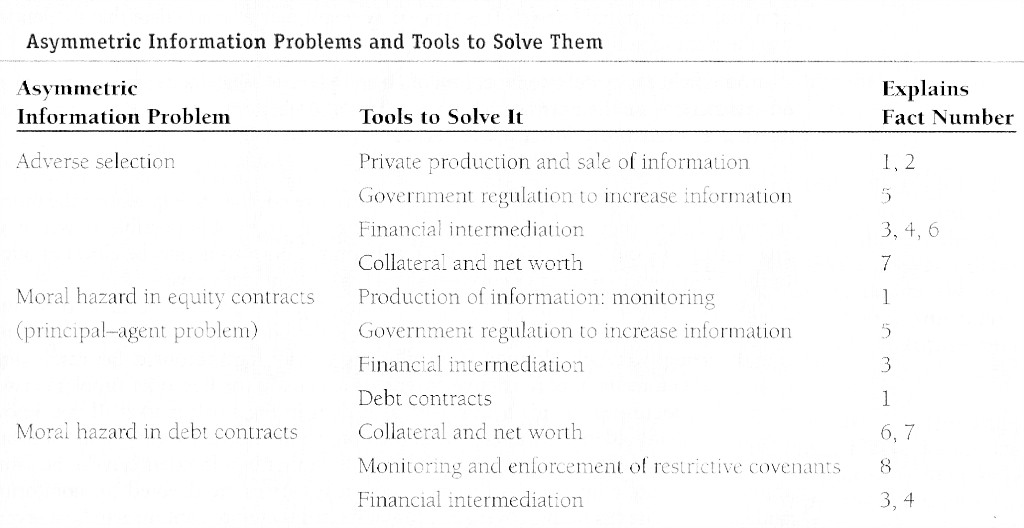
\includegraphics[scale=0.5]{./imgs/81.jpg}

\sh{Financial Development and Economic Growth Problems}
\ra The institutional environment of a poor legal system
\ra Weak accounting standards 
\ra Inadequate government regulation
\ra Government intervention through directed credit programs and state ownership of banks

%%%%%%%%%%%%%%%%%%%%%%%%%%%%%%%%%%%%%%%
\sh{Chapter 9: Financial Crises in advanced economies}
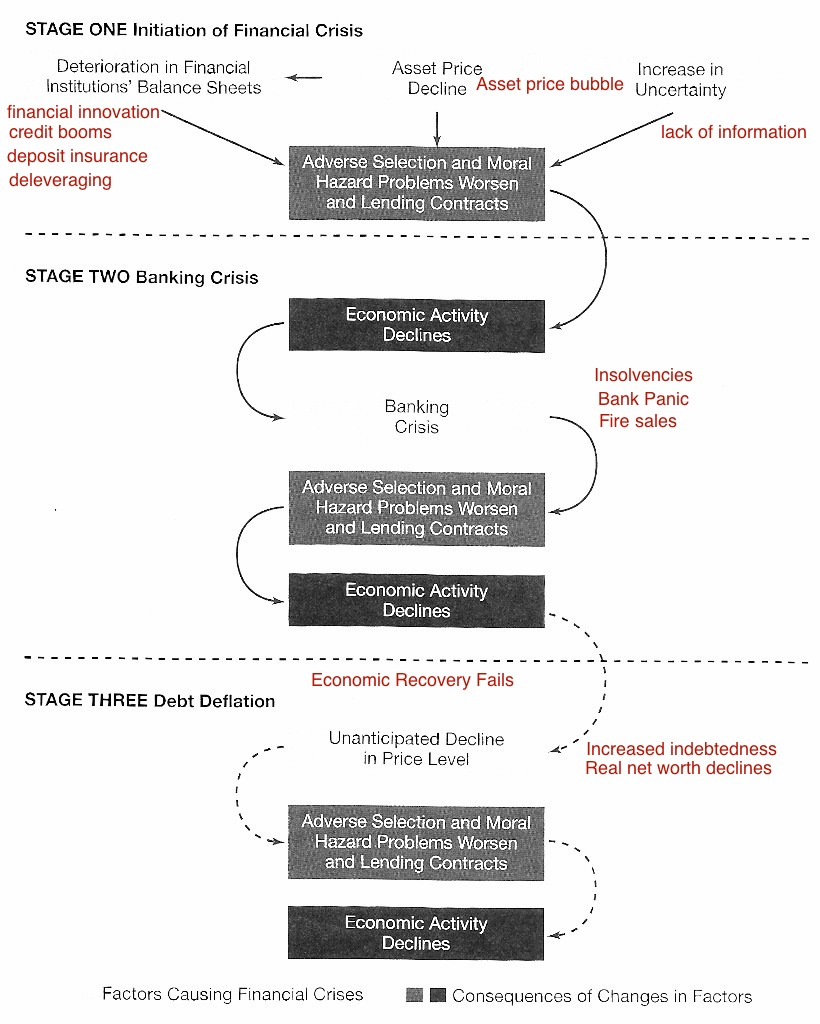
\includegraphics[scale=0.5]{./imgs/91.jpg}

\ssh{Great Depression}
\rn{1} Stock market crash 
\rna Stock market in a boom
\rna Fed was tightening monetary policy.
\rna Stock market crashed
\rna Stocks temporarily recovered part of their losses.
\rn{2} Bank panics
\rna Severe drought lead to large losses on farm mortgages.
\rna Substantial withdrawals from banks lead to bank panic.
\rna Fed did not act and many banks failed.
\rn{3} Continuing decline in stock prices.
\rna Stock fell to 10\% of their value from peak.
\rna Increased uncertainty lead to moral hazard and adverse selection problems
\rna Lending contracted
\rna Increased interest spread.
\rn{4}Debt deflation
\rna Large decline in price level
\rna Short circuited normal recovery process
\rna Increased indebtedness 
\rna Net worth decreases.
\rna Prolonged contraction increased unemployment
\rn{International Dimensions}
\ra Bank panics spread to rest of world
\ra Decreased imports
\ra Worldwide depressions lead to rise of fascism and WW2.

\ssh{Global Financial Crisis 07-09}
Causes
\rn{1} Financial Innovation in Mortgagee markets 
\rna High risk subprime mortgages because of lower transaction costs, computer technology, credit scores and securitisation.
\rna Bundled into mortgage-backed securities, most notorious CDO's
\rna Increased complexity of structured products lead to asymmetric information problems.
\rn{2} Agency problems in the mortgage markets
\rna Originate-to-distribute agency problem
\rna Mortgage brokers did not act in the best interest of investors, due to fees earned.
\rna Risk takers lined up for easy home loans
\rna Banks also suffered from agency problems due to fees
\rna Insurance companies had conflicts of interest on insurance contracts for defaults (credit default swaps) due to large fees.
\rn{3} Asymmetric information and credit-rating agencies.
\rna Advised clients on how to structure complex financial instruments and at the same time they were rating the identical products.
\rna Conflict of interest on fees earned, lacked incentive to rate accurately.

Effects
\rn{1} Residential housing prices: boom and bust
\rna Booming housing prices fuelled by low inters rats and foreign cash flows in subprime mortgage market.
\rna Large amounts of re-mortgaging, and lower house prices lead to value of houses below mortgage value
\rna Increased incentive to just walk away and increased defaults on loans  leading to millions of foreclosures.
\rn{2} Deterioration of finical institutions balance sheets
\rna Value of mortgage backed securities fell leaving banks with lower value of assets and lower net worth
\rna Banks started to de-leverage, selling assets and restricting lending 
\rna Increased financial frictions.
\rn{3} Run on the shadow banking system
\rna Large runs on hedge funds, investment banks and other nondepository institutions.
\rna Increase collateral requirements led to a vicious cycle of fire sale of assets and declining prices. 
\rna Consumption and expenditure declined and the economy contracted.
\rn{4} Global financial markets
\rna Run on shadow banks became worse international
\rna Banks hoarded cash and would not lend to one another
\rna Banks and institutions in Europe started to fail.
\rn{5} Failure of high-profile firms
\rna Bear Stearns sale to J.P Morgan
\rna Fed bailout of Fannie Mae and Freddie Mac
\rna Lehman Brothers bankruptcy
\rna Merrill lynch sale to Bank of America
\rna Government bailout of AIG for losses on credit default swaps.

Height of crisis
\ra Bailout packages 
\ra Increased credit spreads
\ra Stock market crash accelerated
\ra Real GDP declined
\ra Unemployment went up

Government intervention and recovery
\ra Smaller in magnitude than Depression because of massive interventions by governments to prop up financial markets and stimulate economy.
\ra Massive bailouts
\ra Temporary increase of federal deposit insurance limit.
\ra Stocks prices increased
\ra Credit spread began to fall
\ra Slow pace of recovery.

\ssh{Extra Points}
\ra When an asset-price bubble bursts and asset prices realign with fundamental economic values, there is a resulting decline in the net worth of firms and firms have incentives to take on risk at the lender's expense.
\ra  An unanticipated decline in the price level leads to firms' real burden of indebtedness increasing. The resulting decline in a firm's net worth increases adverse selection and moral hazard problems facing lenders.
\ra When a domestic firm's debt contracts are denominated in foreign currency, and when there is an unanticipated decline in the value of the domestic currency, then the debt burden of the firm increases.
\ra  A failure of a major financial institution, which leads to a dramatic increase in uncertainty in financial markets, makes it hard for lenders to screen good from bad credit risks. The resulting inability of lenders to solve the adverse selection problem makes them less willing to lend. 
\ra  Individuals and firms with the riskiest investment projects are those who are willing to pay the highest interest rates. If increased demand for credit drives up interest rates sufficiently, good
credit risks are less likely to want to borrow while bad credit risks are still willing to borrow. 
\ra When there is weak bank regulation and supervision, then financial institutions will take on excessive risk because market discipline is weakened by the existence of a government safety net.

%%%%%%%%%%%%%%%%%%%%%%%%%%%%%%%%%%%%%%%
\sh{Chapter 10: Financial crises in emerging market economies}
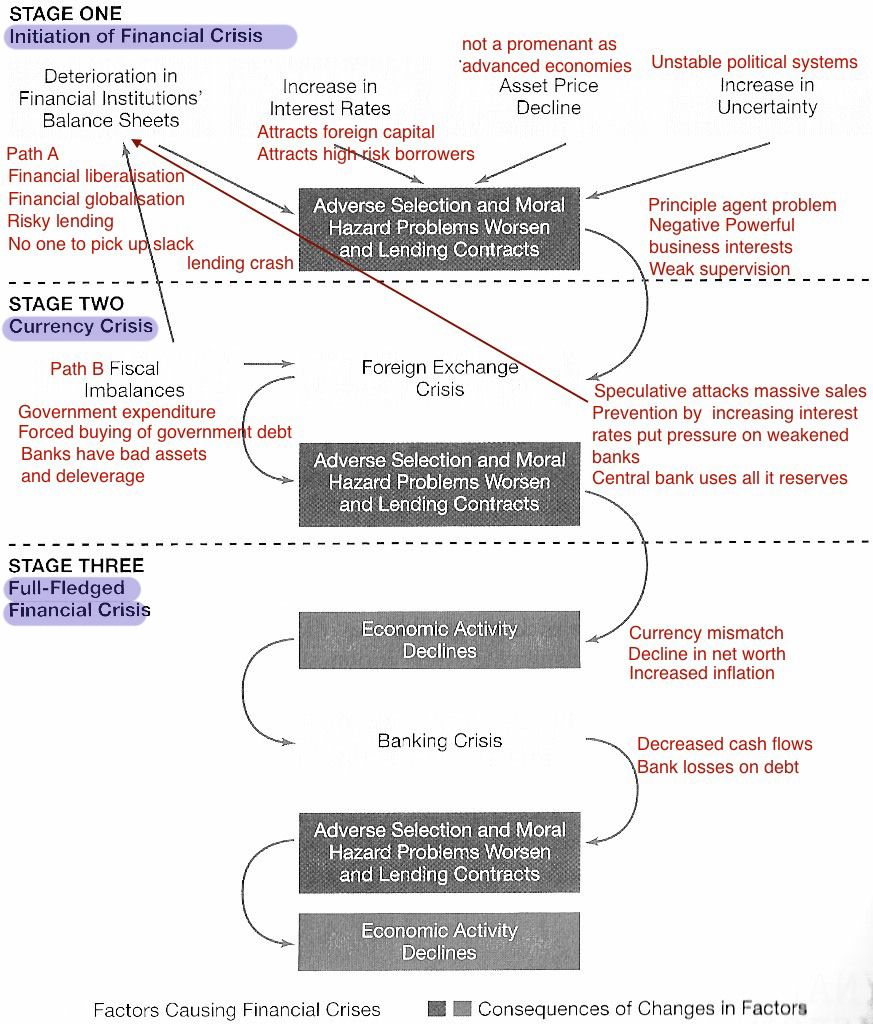
\includegraphics[scale=0.5]{./imgs/101.jpg}

%%%%%%%%%%%%%%%%%%%%%%%%%%%%%%%%%%%%%%%
\sh{Chapter 11: Banking and the management of financial institutions}

\ssh{The bank balance sheet}
\ra Total assets = total liabilities + capital
\ra Profits on interest from assets exceeding interest on liabilities + costs.
Liabilities (sources)
\ra Banks acquire funds by selling or issuing liabilities
\rn{1} Checkable Deposit and money market accounts. Payable on demand. Lowest-cost (interest payments, administration, advertising and branches) source of bank funds.
\rn{2} Nontransaction deposits. Largest source of bank funds. Higher interest no checks. (savings accounts, certificates of deposit,  and negotiable certificates of deposit )
\rn{3} Borrowings. Loans from Fed, other banks and corporations.
\rn{4} Bank capital. Banks net worth. Sales of equity. Cushion against drop in assets.
Assets (uses)
\rn{1} Reserves. Vault cash + Reserves at fed (required reserves + excess reserves)
\rn{2} Cash items in process of collection. 
\rn{3} Deposits at other banks. 
\rn{4} Securities. Short-term government securities are secondary reserves.
\rn{5} Loans. Primary profits. Lack of liquidity and high default risk means higher interest earned on loans.
\rn{6} Other assets. Bank buildings, computers, equipment.

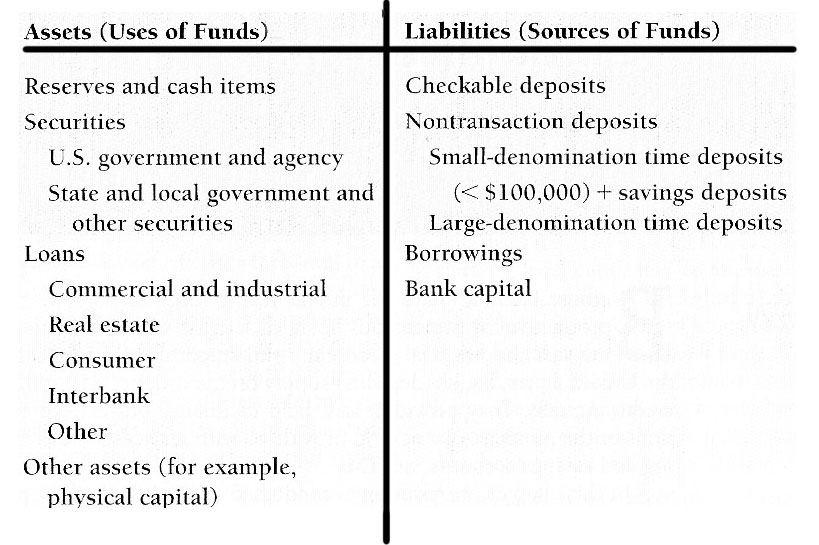
\includegraphics[scale=0.5]{./imgs/111.jpg}

\ssh{Basic banking}
\ra General profits are from asset transformation. (Selling one type buying another) 
\ra Borrows short and lends long.
\ra T-account. Simplified balance sheet with lines in the form of a T, and lists changes that occur in balance sheet items starting from some initial position.
\ra When a bank receives additional deposits it gains an equal amount of reserves and vice versa.
\ra 5 C's
\rn{1} Character
\rn{2} Capacity (ability to pay)
\rn{3} Collateral
\rn{4} Conditions (local and national economy)
\rn{5} Capital (net worth)

\ssh{General principles of bank management}

{\bf Liquidity management}
\ra Acquisition of sufficiently liquid assets to meet the bank's depositor obligations
\ra If a bank has ample excess reserves a deposit outflow does not necessitate changes in other parts of the balance sheet.
\ra To Eliminate required reserve shortfalls.
\rn{1} Borrow from other banks or corporations. Incurs interest costs.
\rn{2} Sell some securities. Brokerage and transaction costs. 
\rn{3} Borrowing from central bank. Cost is discount rate.
\rn{4} Reducing loans. Most costly as antagonises customers.
\ra Excess reserves are insurance against the cost associated with deposit outflows.
{\bf Asset management}
\ra Purse acceptable risk policy. Low rate of default and diversifying.
\rn{1} Find borrowers who will pay high interest rates and not default
\rn{2} Purchase securities with high returns and low risk 
\rn{3} Diversification
\rn{4} Holding liquid securities to meet reserve requirements.
{\bf Liability management}
\ra Acquire funds at low cost
\ra Selling securities other than checkable deposits.
{\bf Capital adequacy management}
\ra Amount of capital the bank should maintain, and acquire needed capital.
\rn{1} Prevent bank failure
\rn{2} Returns for the owners. ROE = ROA x EM. EM (equity multiplier) = $\frac{\text{assets}}{\text{equity capital}}$ Given the return on assets, the lower the bank capital the higher the return for the owners of the bank. Bank might not want to hold too much capital.
\rna Trade-off between safety and returns to equity holders. Bank managers must decided how much of the increased safety that comes with higher capital they are willing to trade off against the lower return on equity that comes with higher capital.
\rn{3} Bank capital requirements by authorities.

\ssh{Strategies for managing bank capital}
\ra To lower the amount of capital relative to assets an raise equity multiplier (smaller valuer).
\rn{1} Stock buy back
\rn{2} Reduced retained earnings by paying higher dividends
\rn{3} Keep bank capital constant but increase asset transformation.
\ra To raise the amount of capital relative to assets an decrease equity multiplier (larger value).
\rn{1} Issue equity
\rn{2} Reduce bank dividends.
\rn{3} Keep bank capital constant but make fewer loans or sell securities and then reduce liabilities.
\ra A shortfall of bank capital is likely to lead to a bank reducing its assets and therefore a contraction in lending.

\ssh{How a capital crunch caused a credit crunch during the Global Financial Crisis}
\ra Shortfalls of capital (losses on mortgage back securities) therefore sale of assets.
\ra Difficult to raise new capital so tightened lending standards and reduced lending.

\ssh{Managing credit risk}
\de{Screening and monitoring}

\rn{1} Screening: Collecting information about prospective borrowers and making judgement calls. Statistics and personal information.
\rn{2} Specialisation in lending. Concentrating lending on firms in specific industries, banks become more knowledgable about specific industries and better able to predict default risk.
\rn{3} Monitoring and enforcement of restrict covenants. Provisions in loan contract restricting risky activities, must be monitored for compliance.

\de{Long-term customer relationships}
\ra Analysis of past activity
\ra Lower costs of monitoring
\ra Easier to obtain loans for borrowers.
\ra Helps with unanticipated moral hazard contingencies.

\de{Loan commitments}
\ra Commitment to a commercial customer to provided loans up to a given amount for a specified future period of time at market interest rates.
\ra Advantage for firms as a source of credit when needed.
\ra Promotes long-term relationships.

\de{Collateral and compensating balances}
\ra Compensating balances: A required minimum cash balance in checking account as collateral. Also Allows bank to monitor account for activity.

\de{Credit rationing}
\ra Refusing loans of any amount. Reduces adverse selection as higher inters rates only attract riskier borrowers.
\ra Restricting size of loan to less than amount wanted. Reduces moral hazard.  More borrowers repay their loans if they are small.

\ssh{Managing interest rate risk}
\ra Rate-sensitive assets/liabilities are short-term.
\ra If a bank has more rate-sensitive liabilities than assets, a rise in interest rates will reduce bank profits and a decline in interest rates will raise bank profits.
\de{Gap and duration analysis}
\ra Gap analysis = rate-sensitive assets - rate-sensitive liabilities X change in interest rate. 
\ra Duration analysis examines the sensitivity of the market value of bank's total assets and liabilities to changes in interest rates.

\ssh{Application: strategies for managing interest rate risk}
\ra Shortening or lengthening duration of banks assets to increase/decrease sensitivity to interest rate changes
\ra Can be costly.

\ssh{Off-balance-sheet activities}
\de{Loan sales} (Secondary loans)
\ra Sale of all or part of the cash stream from a specific loan
\ra Removes loan as an asset from the balance sheet
\ra Sold at a higher amount to earn profit

\de{Generation of fee income}
\ra Providing specialized services such as  foreign exchange services, servicing mortgage backed securities, guaranteeing debt securities.
\ra Providing backup credit such as overdrafts
\ra Off balance sheet activities increase bank's exposure to risk.

\de{Trading activities and risk management techniques}
\ra Trading in debt options, interest-rate swaps and financial futures.
\ra Trading in foreign exchange.
\ra Primary done to reduce risk but speculative trading can lead to large losses and bank insolvencies.
\ra Principle agent problem is huge given the large amount traders have at their disposal and mangers need to implement restrictions and conduct Domesday stress tests.

%%%%%%%%%%%%%%%%%%%%%%%%%%%%%%%%%%%%%%%
\h{Part 4}
\sh{Chapter 14: Central banks: a global perspective}
\ssh{Central Bank Independence:}
\de{FOR:} 
\ra Political pressures would impart an inflationary bias due to their short-term focus on winning the next election; this could lead to a political business cycle, with expansionary policy just before an election and contraction policy after.
\ra It could also be used to fund budget deficits and increase inflation.
\ra Politicians also lack the ability to control monetary policy, and the agency problem is far worse for politicians as they have fewer incentives to act in the public interest.
\ra Independent central banks can pursue politically unpopular policies.
\ra Empirical evidence suggest Independence is best for targeting inflation but central banks should be accountable to parliament.

\de{AGAINST:}
\ra Undemocratic to be controlled by a few elites, with a lack of accountability. 
\ra There needs to be a coordinated effort between fiscal and monetary policy to reduce cross purposes.
\ra Central banks may pursue narrow self interests and can be bureaucratic. 
\ra Does not always use its freedom well, and can fail to act when required.
\ra Can be used as a whipping boy to take heat of politicians.


\ssh{Can monetary policy help to alleviate SA unemployment problem?}
\ra No, Monetary policy is an ineffective tool to achieve this goal, reason why
\rn{1} South Africa's high level of unemployment is mainly a structural problem
\rna Most unemployed are unskilled workers and businesses demand skilled workers
\rna Structural problems of a long term nature are best solved by long term structural solutions.
\rna Such as a good school system, development of worker skills and entrepreneurship.
\rn{2} The economies of countries that have a lower inflation rate generally perform better.
\rna Lowering interest rates increases inflation and lowers long term economic growth.
\rna In the long term, there is no trade-off between price stability and growth
\rn{3} Lower interest rates increase disposable income of households and increases borrowing, increasing aggregate demand and consumption. However 
\ra little impact on unemployment if consumption is on imports
\ra in SA production is not very sensitive to interest rates
\ra even if lower interest rates increase production, it will not necessarily affect employment
\ra More likely that output and employment will react to medium and long term interest rates and not to changes in the short term repo rate.
\rn{4} Everybody can gain by low inflation as the unemployed and poor are impacted the most. 
\rn{5} Lower interest rates might lead to a depreciation of the value of the Rand, increasing the price of imports and raising inflation.
\rn{6} The real interest rate may be low.
\ra The best contribution the SARB's monetary policy can make is to maintain price stability and contain cyclical variation in production employment levels. This creates favourable conditions for sustainable growth in income and employment.

\ssh{The South African Reserve Bank (SARB)}
\de{6 Main Functions}
\rn{1} Sole right to issue cash or currency
\rna Controls SA Mint Company which issues coins and owns SA Bank Note Company which prints banknotes.
\rna New currency is printed to serve the needs of the public. 
\rna The relatively small net income from printing currency accrues to government
\rna Because the printing of new currency generates revenue for the government, it calls for care and restraint, otherwise hyperinflation will occur.

\rn{2} Clearing and the settlement of interbank obligations
\rna Cheques and electronic payments are cleared centrally by the SARB (through the Automated Clearing Bureau)
\rna Settlement is the final discharge of an obligation of one bank in favour of another (A at bank AA writes cheque to pay B at bank BB), by means of the accounts the banks hold with the SARB.
\rna The SARB also oversees the safety and soundness of the payment system through the introduction of settlement risk reduction measures.

\rn{3} Banker for and supervisor of other banks and lender of last resort
\rna Provides accommodation to banks on a daily basis when they experience liquidity shortages 
\rna Holds the statutory cash reserves 
\rna To maintain sound and effective banking practices in the interest of depositors and the economy.

\rn{4} Formulation and implementation of monetary and exchange rate policy
\rna Politically sensitive 
\rna Refinancing or accommodation system where banks are forced into a liquidity shortage and must borrow from SARB at the set repo rate, this then influence the level of all interest rates and hence all participants in the economy.
\rna 

\rn{5} Banker for government
\rna Administering the auctions of government bonds and treasury bills
\rna Participating in National Treasury's debt management meetings 
\rna managing the flow of government funds in the money market

\rn{6} Custodian of gold and other foreign exchange reserves
\ra SARB manages these reserves against international uncertainty, external shocks and exchange rate volatility.

\ssh{Is the SARB independent?}
\ra SARB does not have goal independence and cannot set objectives on its own as the inflation target is set in consultation between the Governor of the SARB and the Minister of Finance. Not necessarily bad as reducing inflation needs the support of government, firms and labour.
\ra SARB has operational (instrument) independence in the choice of instruments it uses and the autonomy to adjust such instruments.
\ra Independence of the SARB is legally established in terms of the Constitution
\ra SARB is accountable to Parliament via the Minister of Finance
\ra The Bank must submit a monthly statement of its assets and liabilities and an annual report to Parliament.
\ra The governor of the SARB also frequently explains the SARB's policy stance in the media.
\ra President appoints the governor and three deputy governors for five-year terms implies SARB may not be completely isolated from political influences.
\ra SARB is financially independent of government
\ra SARB accrues a large surplus net interest income which is paid to government. 
\ra Its operations are not profit driven nor financially constrained by government.

\sh{Chapter 15: The money supply process}

\ssh{Fed's balance sheet}
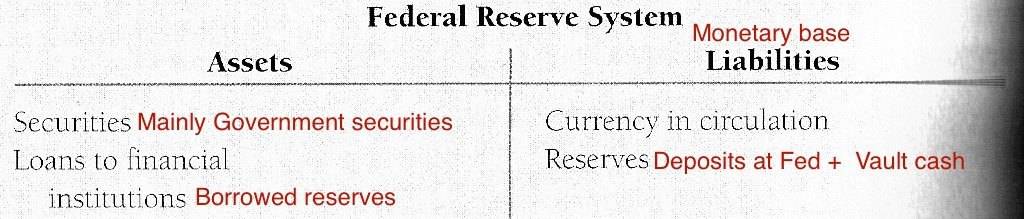
\includegraphics[scale=0.4]{./imgs/152.jpg}

\ssh{Control of the monetary base}
\ra Monetary base (high-powered money) $MB=C+R$
\ra Fed controls monetary base through purchases or sales of securities in the open market and discount loans to banks.
\ra The effect of an open market purchase on reserve depends on whether the seller of the bonds keeps the proceeds from the sale in currency or in deposits
\ra The effect of an open market purchase always increases the monetary base.
\ra The effect of open market transactions on the monetary base is much more certain that the effect on reserves.
\ra Shifts from deposits in currency do not change the monetary base.
\de{Other factors affecting monetary base}
\rn{1} {\bf Float} temporary increase in monetary base from Fed's check-clearing process (crediting bank A before debiting Bank B)
\rn{2} Treasury Deposits 
\rn{3} Intervention in foreign exchange markets.
\ra Nonborrowed monetary base (tight control) = monetary base - borrowed reserves (less control). $MB_n = MB - BR$
\ra Although float and treasury deposits undergo substantial short-run fluctuations, they do not prevent the Fed from actively controlling it.

\ssh{Multiple deposit creations}
\ra  When the Fed supplies the banking system with \$1 of additional reserves, deposits increase by a multiple of it.
\ra A bank cannot safely make a loan for an amount greater than the excess reserves it has before it makes the loan.
\ra Whether a bank chooses to use its excess reserves to make loans or to purchase securities, the effect on deposit expansion is the same.
\ra A single bank cannot by itself generate multiple expansions of deposits, but the banking system as as whole can.
\ra The multiple increase in deposits generated from an increase in the banking system's reserves is called the simple deposit multiplier. $\Delta D = \frac{1}{rr} \times \Delta R$
\rna Deriving: $RR=R$ (no excess reserves), $RR= rr \times D$ substitute into first gives $rr \times R =R$ divide by $rr$ and take change in both sides yields formula.
\ra Deposit creation will l stop only when excess reserves in the banking system are zero, equilibrium, and therefore a given level of reserves in the banking systems determines the level of checkable deposits.
\de{Critique of the simple model.}
\ra Currency has no multiple deposit expansions while deposits do, therefore if proceeds from loans are kept as currency then deposits will not increase as much as model predicts, i.e. does not account for deposits-ratio $c=\frac{C}{D}$
\ra If banks choose to hold on to all or some of their excess reserves, the full expansion of deposit creation does not occur, i.e. does not account for excess-reserves ratio $e=\frac{ER}{D}$
\ra Depositors decisions on how much currency to hold and bankers decisions on the amount of excesses reserves should be taken in to account.
\ra Static model that ignores the steps over time of the deposit creation process.

\ssh{Factors that determine money supply}
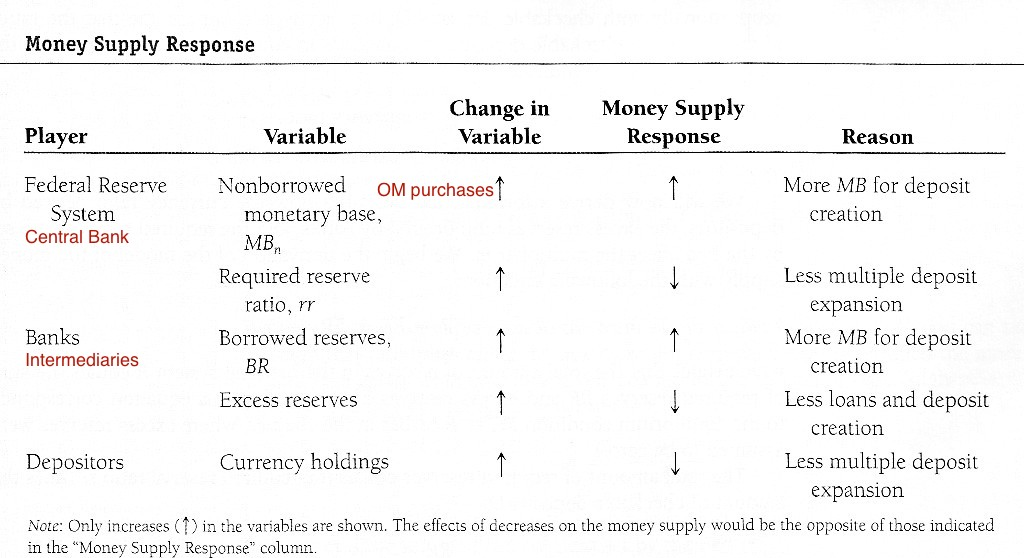
\includegraphics[scale=0.5]{./imgs/151.jpg}

\ssh{Money multiplier}
\ra  $R = RR + ER $ (equilibrium) (ER = excess reserves) (1)
\vspace{6pt}
\ra  $RR = rr \times D$ \quad (D = checkable deposits) (2)
\vspace{6pt}
\ra  Substitute 2 into 1, $R = (rr \times D) + ER$ ($rr < 1)$
\vspace{6pt}
\ra  $MB = R + C = (rr \times D) + ER + C$
\vspace{6pt}
\ra  Given currency ratio $c=\frac{C}{D}$ and excess reserve ratio $e=\frac{ER}{D}$, then after rearranging ratios $MB = (rr \times D) + (e \times D) + (C \times D) = (rr + e + c) \times D$
\vspace{6pt}
\ra Rearranging gives $D=\displaystyle\frac{1}{rr + e + c} \times MB$ (3)
\vspace{6pt}
\ra Using M1 definition of money $M=D+C$ and using $C = c \times D$ gives $M=D + (c \times D)=(1+c) \times D$ (4)
\vspace{6pt}
\ra Substitute 4 into 3 gives $M=\displaystyle\frac{1+c}{rr + e + c} \times MB$ 
\vspace{6pt}
\ra therefore money multiplier $m=\displaystyle\frac{1+c}{rr + e + c} \times MB$ \quad  ($m > 1$ if $rr < 1$)

\de{Money supply response to changes in the factors}
\ra $M= m \times (MB_n + B)$
\ra level of currency does rise when the monetary base and checkable deposits increase because $c > 0$ 

\ssh{Monetary policy in SA}
\ra SARB does not pay interest on bank reserves and government deposits.
\ra Government transfers from SARB to banks/nonbank accounts increases reserves. 
\ra SARB buying foreign exchange from banks increases bank reserves.
\ra Tax and loan accounts are accounts with the commercial banks, transfers from these accounts to and from SARB are used to manipulate reserves of banks for monetary policy reasons.

\ssh{Money supply in South Africa}
\ra Money supply = cash and deposits of the nonbank public.
\ra Money supply increases because of:
\rn{1} There is a net increase in the loans the banks grant to the nonbank public.
\rn{2} There is a net increase in assets (mostly securities) that banks buy from the nonbank public.
\rn{3} There is a net increase in the payments the central bank makes to the nonbank public (open-market purchases from nonbank public)
\rn{4} There is a net increase in the payments the government makes to the nonbank public. (budget deficit)
\rn{5} There is a net increase in the amount of foreign exchange the nonbank public sells to the banks. (surplus on the balance of payments)

\vspace{6pt}
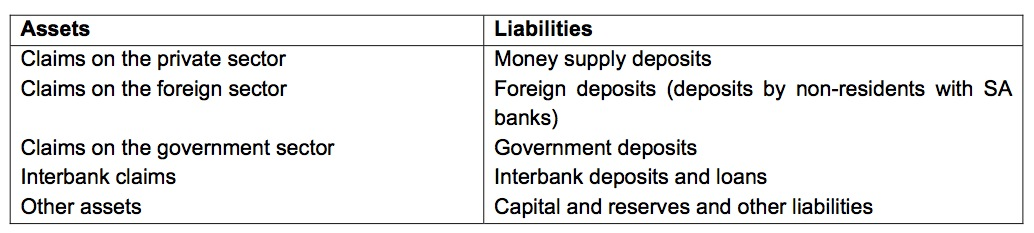
\includegraphics[scale=0.5]{./imgs/153.jpg}

\ssh{Causal direction of money supply process in SA}
\ra Mishkin implies reserve holding leads to deposit creation others argue deposits creation leads to reserve holding.
\ra Commercial banks are dependent on the central bank for their cash reserves and a small part from selling forex.
\ra Central bank functions as the "lender of last resort" and it is compelled to also supply the banking system with its normal cash reserves requirements.
\ra Two strategies to supply the banking system with cash reserves:
\rn{1} Can control amount of cash reserves it provides and allow the cash fund rate (Fed funds rate/ repo rate) to find its own level as determined by the demand for cash reserves.
\rn{2} Can fix the cash funds rate and allow the amount of cash reserves to find its own level, as determined by the demand for cash.
\rna There is only a price constraint (cash fund rate) and no quantity constraint.
\rna No choice but to accommodate fully and unconditionally the banking sector's total demand for cash reserves at that target level.
\rna Individual banks that require a disproportionate amount of cash because they have been  irresponsible, may be refused and allowed to go bankrupt unless they are to big to fail.
\rna Averagely prudent banks are assured of their cash reserves at the prevailing repo rate. 
\rna If banks are equally competitive, they face the same growth in the demand for credit and can issue all their deposits as credit, and obtain their cash reserves from SARB. This implies that deposits lead to cash holdings.
\rna (D → R or M → MB) implies that changes in r, c and e ratios does not cause a change in the impact of R on D.
\rna If banks are assured cash reserves, there is no reason for excess cash reserves. Excess cash reserves are lent to other banks.
\rna Banks only need to keep the required cash reserves as an average over a month period. Removes the need to hold large excess reserves on a daily basis.

%%%%%%%%%%%%%%%%%%%%%%%%%%%%%%%%%%%%%%%
\sh{Chapter 16: The tools of monetary policy}
\begin{center}
  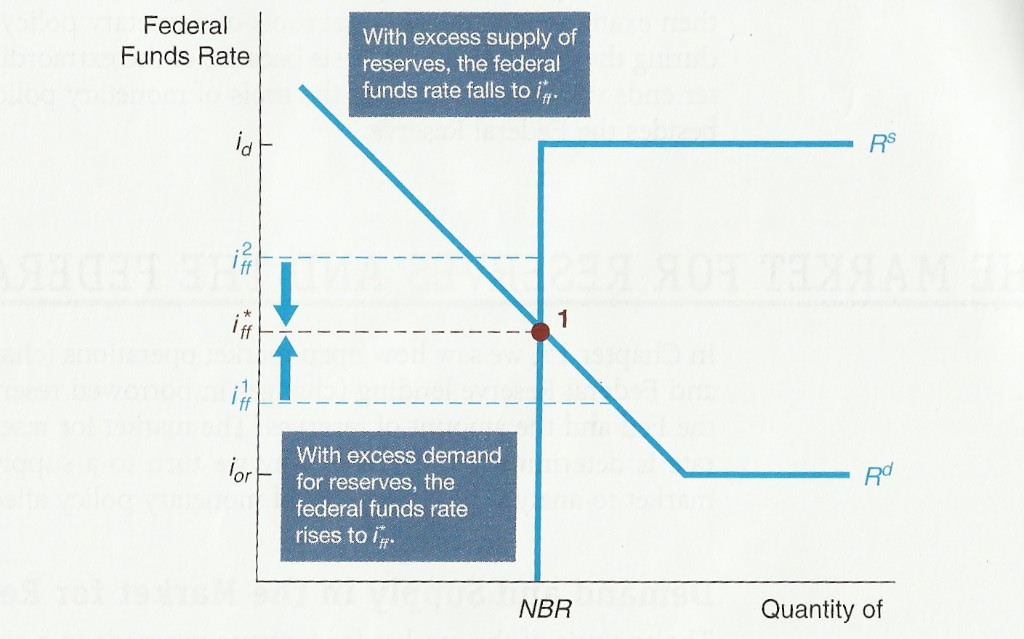
\includegraphics[scale=0.4]{./imgs/chapter16fig1.jpg}
  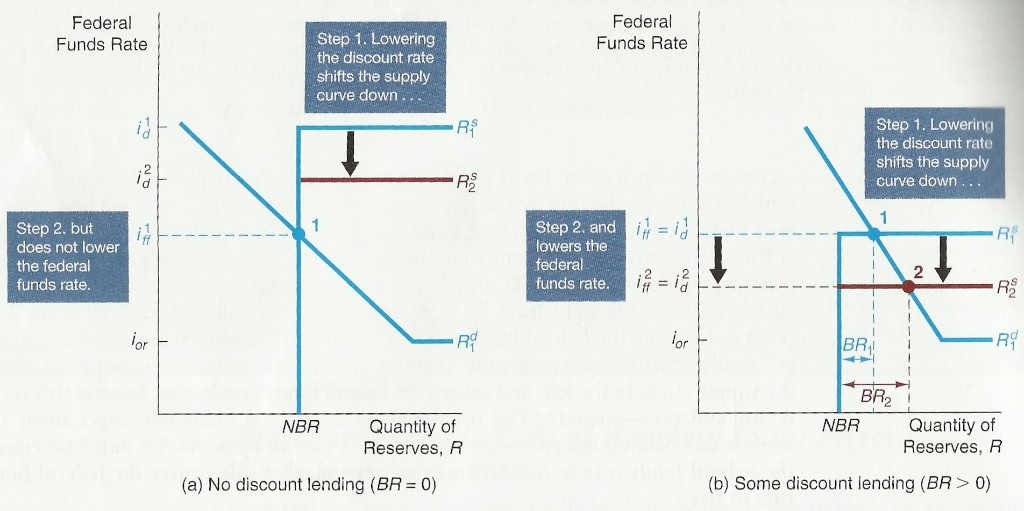
\includegraphics[scale=0.5]{./imgs/chapter16fig3.jpg}
\end{center}

%%%%%%%%%%%%%%%%%%%%%%%%%%%%%%%%%%%%%%%
\sh{Chapter 17: The conduct of monetary policy: Strategy and tactics}
\begin{center}
  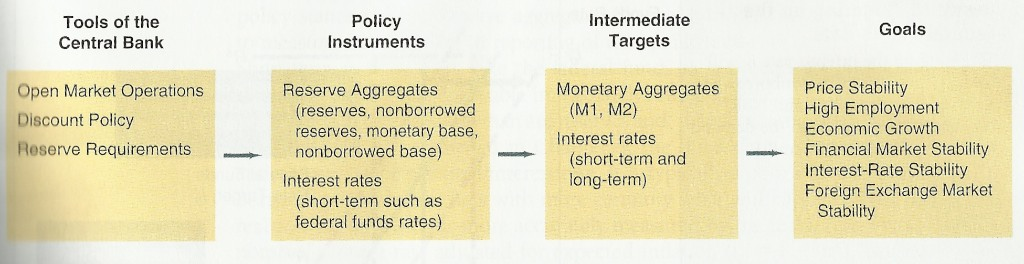
\includegraphics[scale=0.5]{./imgs/chap17fig2.jpg}
  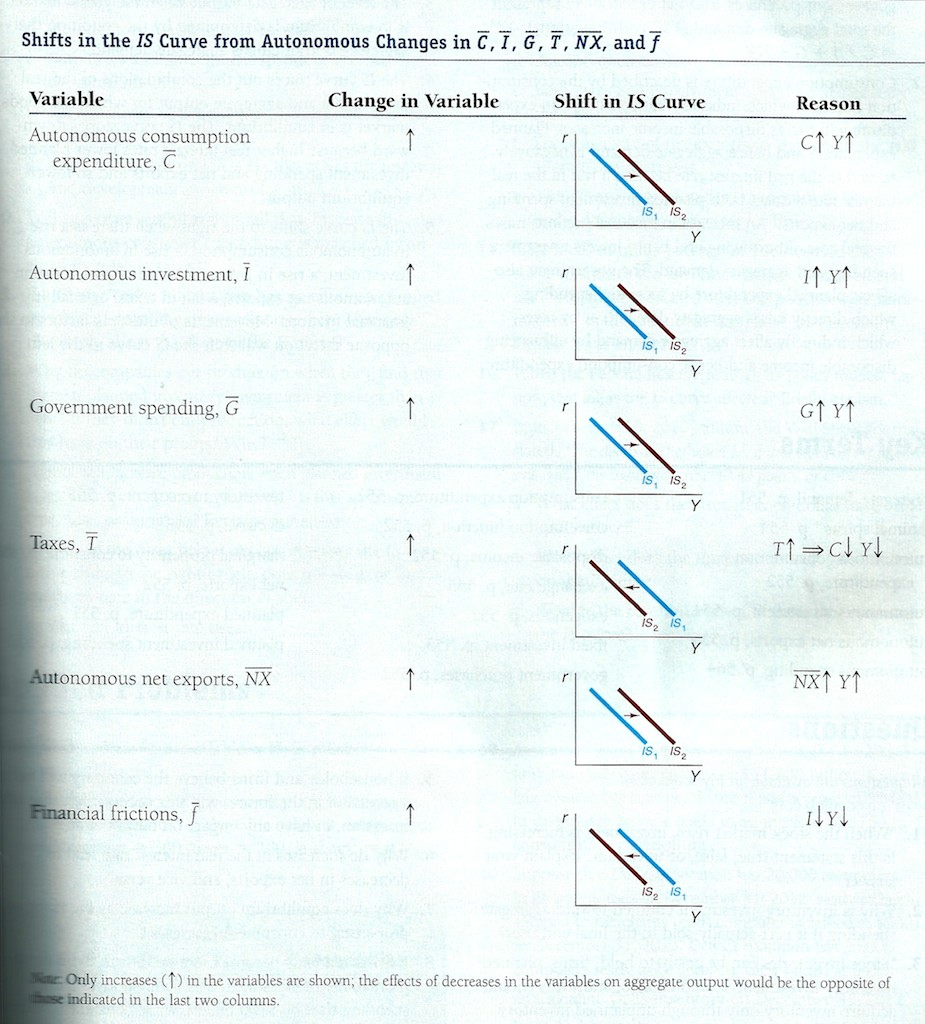
\includegraphics[scale=0.5]{./imgs/c21t1.jpg}
\end{center}


%%%%%%%%%%%%%%%%%%%%%%%%%%%%%%%%%%%%%%%
\h{Part 6}

\sh{Chapter 20: Quantity theory, inflation and the demand for money}
Velocity of Money = $\displaystyle\frac{P \times Y}{M}$ 
Equation of Exchange: $M\times V=P \times Y$
\begin{center}
  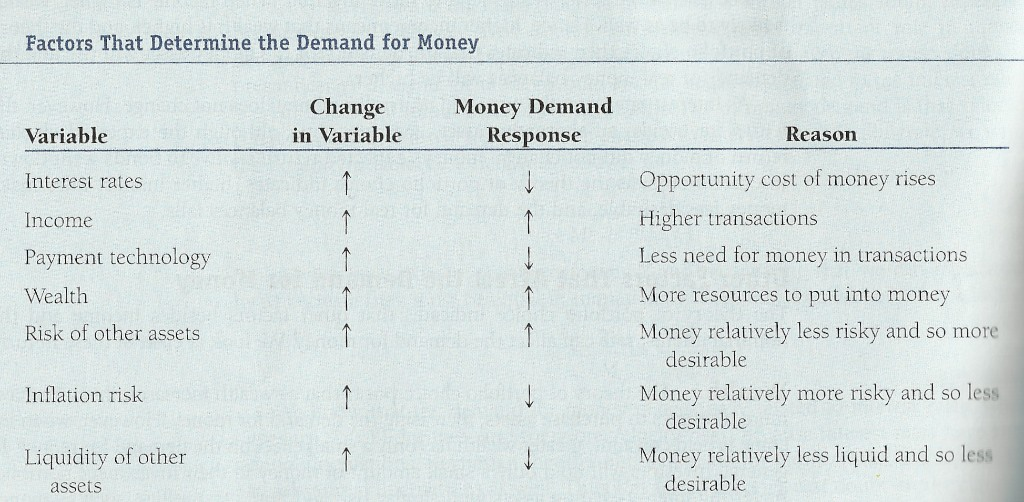
\includegraphics[scale=0.5]{./imgs/c20t1.jpg}
\end{center}

%%%%%%%%%%%%%%%%%%%%%%%%%%%%%%%%%%%%%%%
\sh{Chapter 21: The IS curve}
\begin{center}
  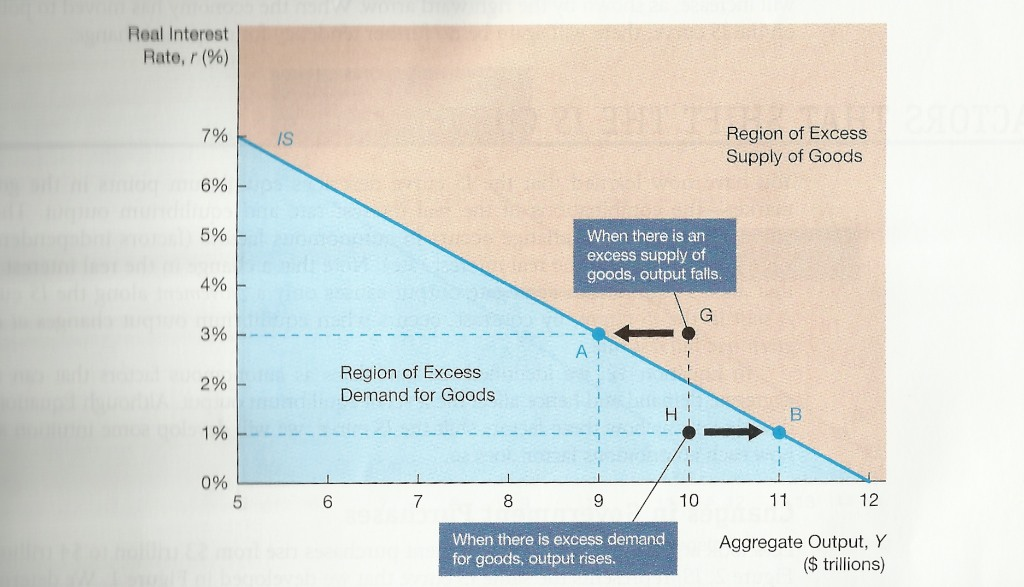
\includegraphics[scale=0.5]{./imgs/c21f1.jpg}
\end{center}

\sh{Chapter 24: Monetary Policy Theory}
\begin{center}
  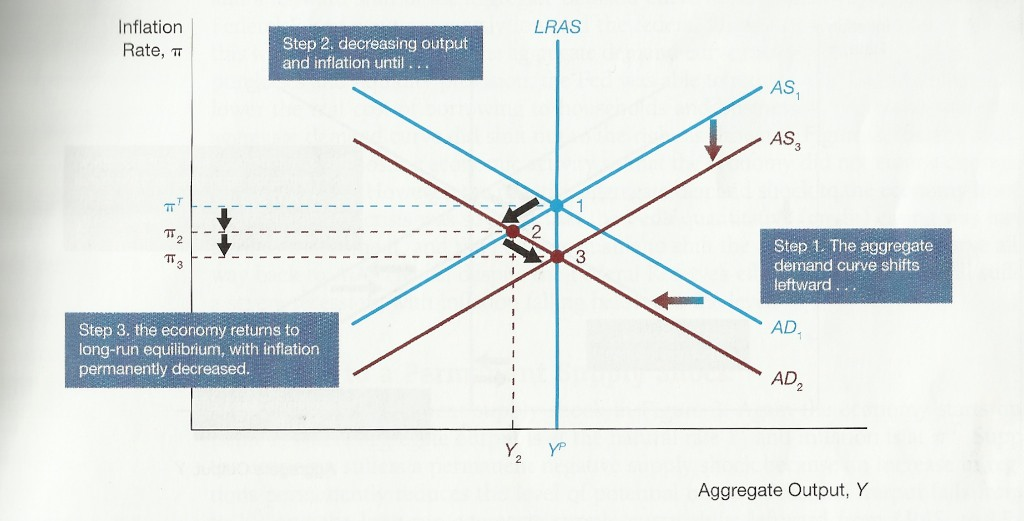
\includegraphics[scale=0.5]{./imgs/c24f1.jpg}
  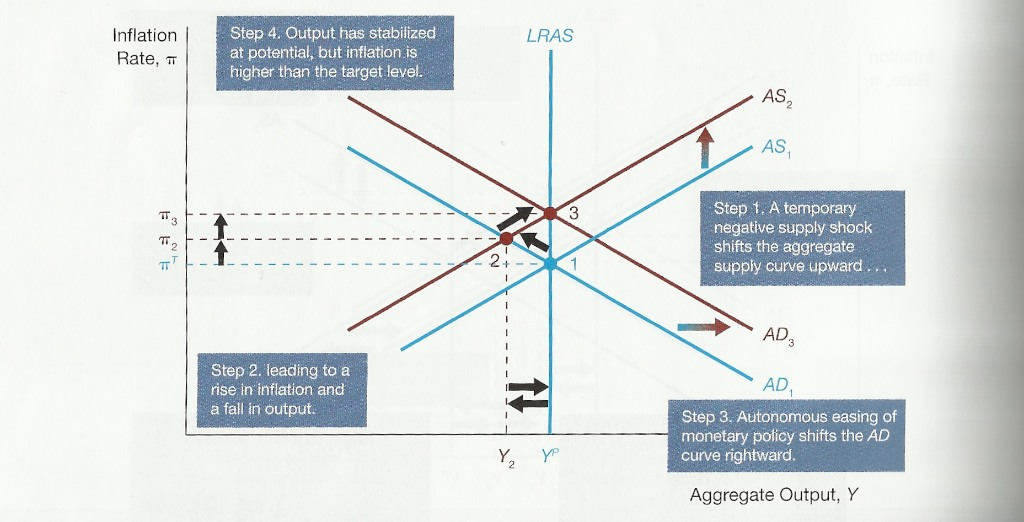
\includegraphics[scale=0.5]{./imgs/c24f7.jpg}
  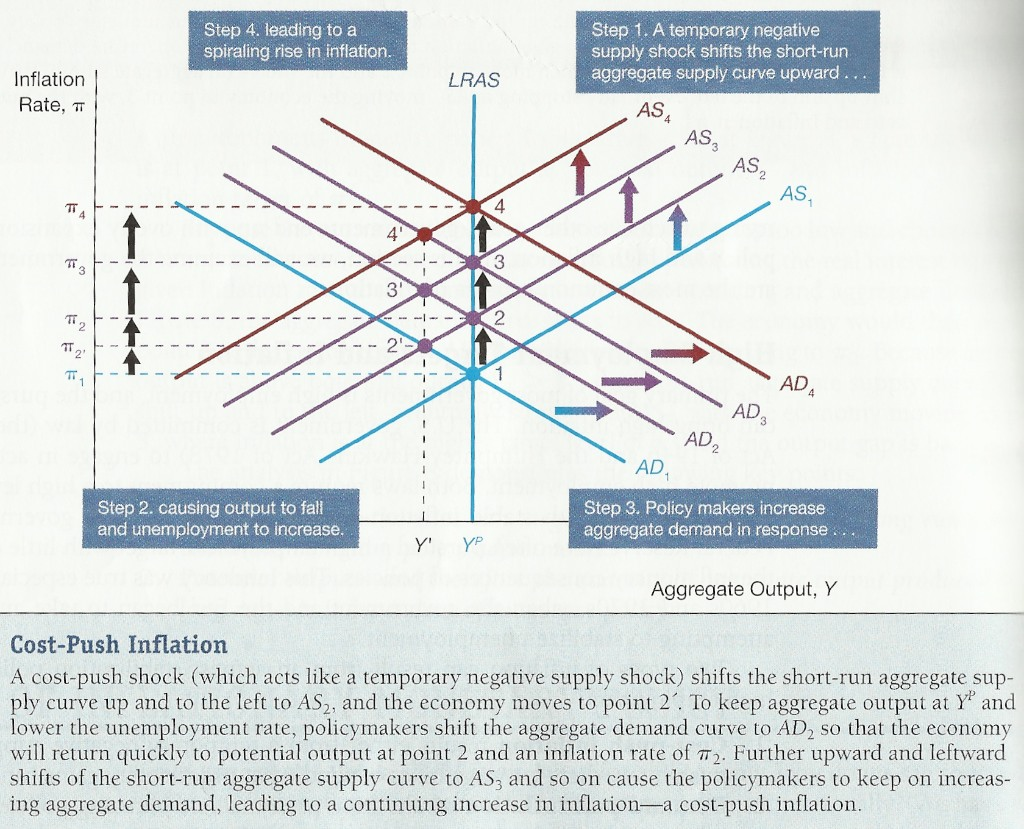
\includegraphics[scale=0.4]{./imgs/c24f9.jpg}
    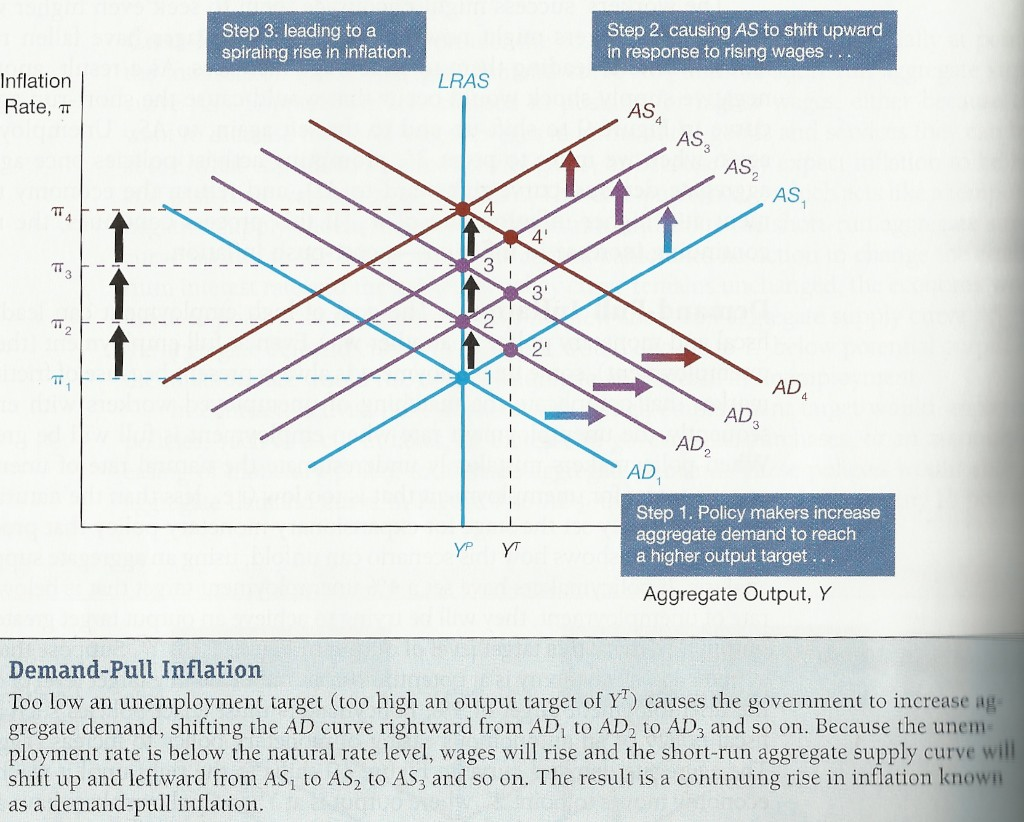
\includegraphics[scale=0.4]{./imgs/c24f10.jpg}
\end{center}
\colorbox{red}{\textcolor{white}{definitely lots of marks here}}

%%%%%%%%%%%%%%%%%%%%%%%%%%%%%%%%%%%%%%%
\sh{Chapter 25: The role of expectations in monetary policy}


%%%%%%%%%%%%%%%%%%%%%%%%%%%%%%%%%%%%%%%
\sh{Chapter 26: Transmission mechanism of monetary policy}
\begin{center}
  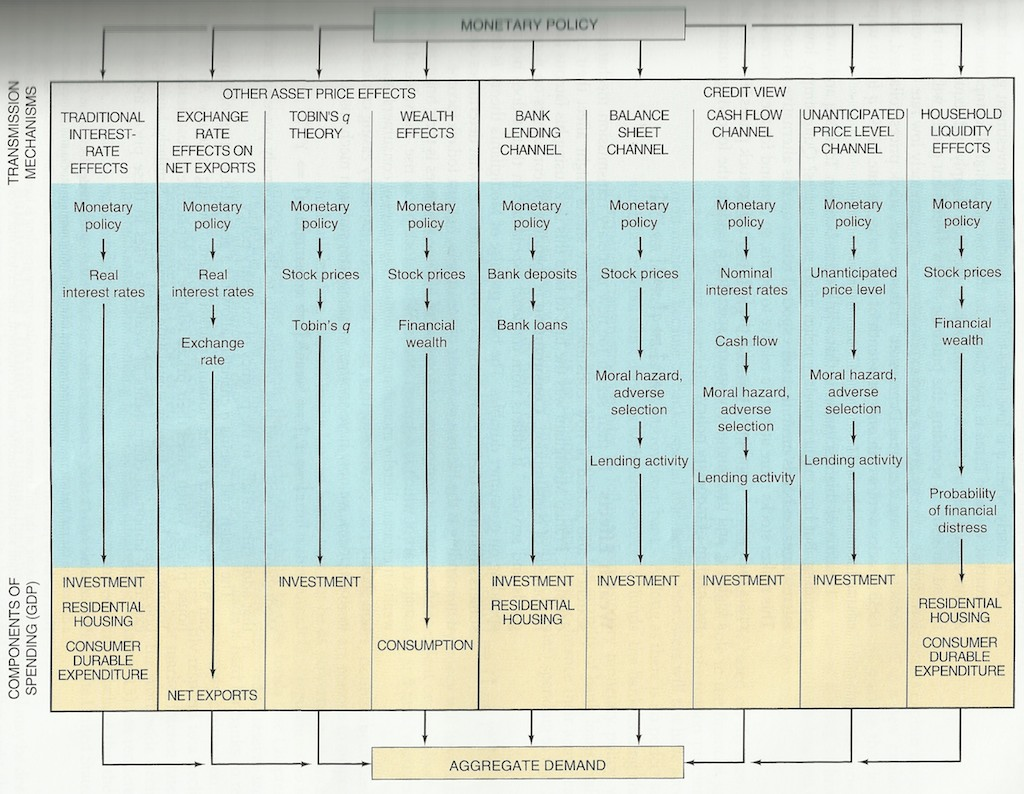
\includegraphics[scale=0.5]{./imgs/c26f1.jpg}
\end{center}

\end{document}
